\documentclass[a4paper,11pt]{article}
%\documentclass[a4paper,twoside,11pt,titlepage]{book}
\usepackage{listings}
\usepackage[utf8]{inputenc}
\usepackage[spanish]{babel}
\usepackage[backend=biber, style=alphabetic]{biblatex} 
\usepackage{amsmath}
\usepackage{amssymb}
\usepackage{algorithm}
\usepackage{algpseudocode}
\usepackage{multirow}

\addbibresource{bibliografia.bib}
%Que no se muestren las imagenes
%\setkeys{Gin}{draft}

% \usepackage[style=list, number=none]{glossary} %
%\usepackage{titlesec}
%\usepackage{pailatino}

\decimalpoint
\usepackage{dcolumn}
\newcolumntype{.}{D{.}{\esperiod}{-1}}
\makeatletter
\addto\shorthandsspanish{\let\esperiod\es@period@code}
\makeatother


%\usepackage[chapter]{algorithm}
\RequirePackage{verbatim}
%\RequirePackage[Glenn]{fncychap}
\usepackage{fancyhdr}
\usepackage{graphicx}
\usepackage{afterpage}



\usepackage{longtable}

\usepackage[pdfborder={000}]{hyperref} %referencia


%Math packages
\usepackage{dsfont}

% ********************************************************************
% Re-usable information
% ********************************************************************
\newcommand{\myTitle}{TFG\xspace}
\newcommand{\myDegree}{Grado en ...\xspace}
\newcommand{\myName}{Eduardo Morales Muñoz\xspace}
\newcommand{\myProf}{Pablo Mesejo Santiago\xspace}
\newcommand{\myOtherProf}{Javier Merí de la Maza\xspace}
%\newcommand{\mySupervisor}{Put name here\xspace}
\newcommand{\myFaculty}{Escuela Técnica Superior de Ingenierías Informática y de
Telecomunicación\xspace}
\newcommand{\myFacultyShort}{E.T.S. de Ingenierías Informática y de
Telecomunicación\xspace}
\newcommand{\myDepartment}{Departamento de ...\xspace}
\newcommand{\myUni}{\protect{Universidad de Granada}\xspace}
\newcommand{\myLocation}{Granada\xspace}
\newcommand{\myTime}{\today\xspace}
\newcommand{\myVersion}{Version 0.1\xspace}



\hypersetup{
pdfauthor = {\myName eedduuy@correo.ugr.es},
pdftitle = {\myTitle TFG},
pdfsubject = {},
pdfkeywords = {palabra_clave1, palabra_clave2, palabra_clave3, ...},
pdfcreator = {LaTeX con el paquete ....},
pdfproducer = {pdflatex}
}

%\hyphenation{}


%\usepackage{doxygen/doxygen}
%\usepackage{pdfpages}
\usepackage{url}
\usepackage{colortbl,longtable}
\usepackage[stable]{footmisc}
%\usepackage{index}

\makeindex
%\usepackage[style=long, cols=2,border=plain,toc=true,number=none]{glossary}
% \makeglossary

% Definición de comandos que me son tiles:
%\renewcommand{\indexname}{Índice alfabético}
%\renewcommand{\glossaryname}{Glosario}

\pagestyle{fancy}
\fancyhf{}
\fancyhead[LO]{\leftmark}
\fancyhead[RE]{\rightmark}
\fancyhead[RO,LE]{\textbf{\thepage}}
%\renewcommand{\chaptermark}[1]{\markboth{\textbf{#1}}{}}
%\renewcommand{\sectionmark}[1]{\markright{\textbf{\thesection. #1}}}

\setlength{\headheight}{1.5\headheight}

\newcommand{\HRule}{\rule{\linewidth}{0.5mm}}
%Definimos los tipos teorema, ejemplo y definición podremos usar estos tipos
%simplemente poniendo \begin{teorema} \end{teorema} ...
\newtheorem{teorema}{Teorema}[section]
\newtheorem{ejemplo}{Ejemplo}[section]
\newtheorem{definicion}{Definición}[section]
\newtheorem{proposicion}{Proposición}[section]



\definecolor{gray97}{gray}{.97}
\definecolor{gray75}{gray}{.75}
\definecolor{gray45}{gray}{.45}
\definecolor{gray30}{gray}{.94}

\lstset{ frame=Ltb,
     framerule=0.5pt,
     aboveskip=0.5cm,
     framextopmargin=3pt,
     framexbottommargin=3pt,
     framexleftmargin=0.1cm,
     framesep=0pt,
     rulesep=.4pt,
     backgroundcolor=\color{gray97},
     rulesepcolor=\color{black},
     %
     stringstyle=\ttfamily,
     showstringspaces = false,
     basicstyle=\scriptsize\ttfamily,
     commentstyle=\color{gray45},
     keywordstyle=\bfseries,
     %
     numbers=left,
     numbersep=6pt,
     numberstyle=\tiny,
     numberfirstline = false,
     breaklines=true,
   }
 
% minimizar fragmentado de listados
\lstnewenvironment{listing}[1][]
   {\lstset{#1}\pagebreak[0]}{\pagebreak[0]}

\newcommand{\bigrule}{\titlerule[0.5mm]}


%Para conseguir que en las páginas en blanco no ponga cabecerass
\makeatletter
\def\clearpage{%
  \ifvmode
    \ifnum \@dbltopnum =\m@ne
      \ifdim \pagetotal <\topskip
        \hbox{}
      \fi
    \fi
  \fi
  \newpage
  \thispagestyle{empty}
  \write\m@ne{}
  \vbox{}
  \penalty -\@Mi
}
\makeatother

\pagenumbering{roman}
\usepackage{pdfpages}
\begin{document}
\begin{titlepage}
 
 
\newlength{\centeroffset}
\setlength{\centeroffset}{-0.5\oddsidemargin}
\addtolength{\centeroffset}{0.5\evensidemargin}
\thispagestyle{empty}

\noindent\hspace*{\centeroffset}\begin{minipage}{\textwidth}

\centering

\includegraphics[width=0.7\textwidth]{Plantilla_TFG_latex/imagenes/logo_ugr.jpg}\\[1.4cm]

\textsc{ \Large TRABAJO FIN DE GRADO\\[0.2cm]}
\textsc{ Doble Grado Ingeniería Informática y Matemáticas}\\[1cm]
% Upper part of the page
% 
% Title
{\huge\bfseries Análisis del algoritmo de gradiente descendente y estudio empírico comparativo con técnicas metaheurísticas\\
}
\noindent\rule[-1ex]{\textwidth}{3pt}\\[3.5ex]

\end{minipage}

\vspace{1cm}
\noindent\hspace*{\centeroffset}\begin{minipage}{\textwidth}
\centering

\textbf{Autor}\\ {Eduardo Morales Muñoz}\\[2.5ex]
\textbf{Directores}\\
{Pablo Mesejo Santiago\\
Javier Meri de la Maza}\\[1cm]
\raggedright
\hspace{3cm}

\includegraphics[width=0.12\textwidth]{Plantilla_TFG_latex/imagenes/fcienciasLogo.png}\hspace{3.5cm}

\includegraphics[width=0.3\textwidth]{Plantilla_TFG_latex/imagenes/etsiit_logo.png} \\[0.1cm]

\centering
\vspace{0.5cm}
\textsc{Facultad de Ciencias \\ Escuela Técnica Superior de Ingenierías Informática y de Telecomunicación}\\
\textsc{---}\\
Granada, \today
\end{minipage}
%\addtolength{\textwidth}{\centeroffset}
%\vspace{\stretch{2}}
\end{titlepage}



%%\newpage
%\thispagestyle{empty}
%\mbox{}
%\newpage

\section*{Declaración de originalidad}

Yo, \textbf{Eduardo Morales Muñoz}, con DNI 77200029T, declaro explícitamente que el presente trabajo, titulado \textit{\textbf{Análisis del algoritmo de gradiente descendente y estudio empírico comparativo con técnicas metaheurísticas}}, y presentado como Trabajo de Fin de Grado (TFG), correspondiente al curso académico 2024-2025, es original, entendida esta, en el sentido de que no han sido utilizadas para la elaboración del trabajo fuentes sin citarlas debidamente.

\vspace{6cm}

\noindent Fdo: Eduardo Morales Muñoz

\vspace{2cm}

\begin{flushright}
Granada a \today.
\end{flushright}

\newpage


D. \textbf{Pablo Mesejo Santiago}, Profesor del Departamento de Ciencias de la Computación e Inteligencia Artificial de la Universidad de Granada.

\vspace{0.5cm}

D. \textbf{Francisco Javier Meri de la Maza}, Profesor del Departamento de Análisis Matemático de la Universidad de Granada.


\vspace{0.5cm}

\textbf{Informan:}

\vspace{0.5cm}

Que el presente trabajo, titulado \textit{\textbf{Análisis del algoritmo de gradiente descendente y estudio empírico comparativo con técnicas metaheurísticas}},
ha sido realizado bajo su supervisión por \textbf{Eduardo Morales Muñoz}, y autorizamos la defensa de dicho trabajo ante el tribunal que corresponda.

\vspace{0.5cm}

Y para que conste, expiden y firman el presente informe en Granada a \today.

\vspace{1cm}

\textbf{Los directores:}

\vspace{5cm}

\noindent \textbf{Pablo Mesejo Santiago \ \ \ \ \ Francisco Javier Meri de la Maza}


\newpage
%\thispagestyle{empty}
%\mbox{}
%\newpage


Yo, \textbf{Eduardo Morales Muñoz}, alumno de la titulación Doble Grado Ingeniería Informática y Matemáticas de la \textbf{Escuela Técnica Superior de Ingenierías Informática y de Telecomunicación de la Universidad de Granada}, con DNI 77200029T, autorizo la ubicación de la siguiente copia de mi Trabajo Fin de Grado en la biblioteca del centro para que pueda ser
consultada por las personas que lo deseen.

\vspace{6cm}

\noindent Fdo: Eduardo Morales Muñoz

\vspace{2cm}

\begin{flushright}
Granada a \today.
\end{flushright}



\newpage




%\newpage
%\thispagestyle{empty}
%\mbox{}
%\newpage

\section*{Agradecimientos}
\addcontentsline{toc}{section}{Agradecimientos}

       \vspace{1cm}


Gracias a mi abuelo, por hacerme ser quien soy ahora. Gracias a mis amigos y mi familia por acompañarme en este largo proceso y ofrecerme el apoyo, espacio y entendimiento. Gracias a mis tutores Javier y Pablo.


%\frontmatter
\tableofcontents
\newpage
%\listoffigures
%\listoftables
%
%\mainmatter
%\setlength{\parskip}{5pt}
\pagenumbering{arabic}
\setcounter{page}{1}
\setcounter{section}{0}
%\section{Introducción}

 %El más común es el aprendizaje supervisado \cite{mitchell1997machine}, donde la tarea $T$ es mapear una función $f$ desde unas entradas $x \in X$ hacia unas salidas $y \in Y$. Las entradas también son llamadas características y las salidas etiquetas. La experiencia $E$ es el conjunto de N parejas $\mathcal{D}=\left \{ (x_n,y_n) \right \} ^{N}_{n=1} $ que llamamos conjunto de entrenamiento. 


%En los problemas de clasificación, la salida es un conjunto no ordenado $Y= \left \{ 1,2,...,C \right \}$ donde sus elementos son denominados clases. Las tareas de clasificación de imágenes tienen un conjunto de imágenes $X$ como entrada, siendo $X=\mathds{R}^D$ donde $D=C \times D_1 \times D_2$. $C$ es el número de canales de la imágen (por ejemplo 3 si es en color RGB y 1 en escala de grises) y $D_1 \times D_2$ las dimensiones en píxeles de las imágenes.

 %Se trata también del enfoque sobre el que más se ha investigado en el aprendizae automático. \footnote{Realizando una búsqueda en Google Scholar obtenemos 6.8M de resultados para \textit{deep learning}, por encima de los 3.21M para \textit{logistic regression}, 5.51M para \textit{linear regression}, 3.58M para \textit{support vector machine} y 0.78M para \textit{gradient boosting}}. 






%Este término muchas veces se confunde con el propio algoritmo de aprendizaje (gradiente descentente), ya que aunque existen otras alternativas para este cálculo como los métodos numéricos 


%En las principales familias de modelos en cuanto a avances y resultados obtenidos como redes neuronales (ya sea convolucionales, recurrentes o con memoria), redes generativas adversarias o \textit{transformers}, el algoritmo de aprendizaje más usado es el descenso de gradiente, por ende en la mayoría está implícito el uso de \textit{backpropagation}.

%



Las metaheurísticas \cite{MHDef} son métodos de resolución que combinan procedimientos de mejora local y estrategias de alto nivel para crear un algoritmo capaz de escapar óptimos locales y desarrollar una búsqueda robusta del espacio de soluciones . Resultan especialmente útiles en problemas donde no existe una heurística específica o ésta es demasiado costosa computacionalmente, ya que pueden alcanzar soluciones cercanas a la óptima con un coste muy reducido. Su uso en el aprendizaje automático es cada vez más extendido, siendo usadas en diferentes tareas como entrenamiento de modelos, selección de hiperparámetros o elección de las arquitecturas de los modelos, con resultados diversos en cada una de estas tareas. 


%Los algoritmos genéticos \cite{MHDef} son una clase de algoritmos metaheurísticos inspirados en el proceso de selección natural y de evolución. Se basan en los principios de herencia, mutación y selección para desarrollar una población de soluciones de manera iterativa. Las soluciones son representadas como individuos o cromosomas, con una estructura dependiente del problema, y se evalúa su calidad con una función objetivo. Son una aproximación flexible y potente a la optimización, resolviendo una amplia gama de problemas de diversos ámbitos como financias, ingeniería o aprendizaje automático. Los algoritmos meméticos \cite{MHDef} son técnicas de optimización metaheurísticas basadas en la combinación de componentes de búsqueda global y local, usando conocimiento específico del problema, a diferencia de los algoritmos genéticos que no la usan. Suelen fundamentarse en estrategias basadas en población donde cada cierto número de generaciones se aplica un algoritmo de búsqueda local.


\subsection{Motivación}

Las redes neuronales profundas han permitido desarrollar modelos con muy buenos resultados en la última década y han favorecido en gran medida el desarrollo de la investigación en el aprendizaje automático. La estrategia más común que se ha tenido de entrenarlas ha sido, y sigue siendo a día de hoy, el algoritmo de gradiente descendente, por lo que están estrechamente relacionadas. La herramienta que hace posible a nivel de eficiencia computacional y escalabilidad el cálculo del gradiente y por tanto el entrenamiento de estos modelos, es \textit{backpropagation}. Aunque se estén desarrollando nuevas estrategias \cite{Metaheuristics_train} para el ajuste de pesos, sigue resultando una piedra angular y su papel en el entrenamiento de modelos desde la década de los 1990s es crucial. Estas nuevas técnicas, principalmente metaheurísticas, todavía no han logrado igualarse a las clásicas en sus resultados y costes computacionales en la tarea del ajuste de pesos, aunque se usan muy satisfactoriamente en otras tareas como la selección de hiperparámetros y arquitecturas de un modelo \cite{MHforNeuralArchAndHyper}.

Algunos problemas importantes abiertos en el campo son:

\begin{itemize}
 %   \item \textbf{Interpretabilidad}: a pesar de su gran rendimiento las redes neuronales profundas carecen totalmente de interpretabilidad, y se están desarrollando técnicas para poder explicar qué decisiones toman los modelos y por qué. \cite{interpr}

    \item \textbf{Estabilidad en el entrenamiento}: los algoritmos de aprendizaje son en general muy sensibles a la elección de los hiperparámetros y la inicialización de los pesos de los modelos, que pueden llevar a problemas de convergencia como desvanecimiento o explosión de gradiente. \cite{stabilityProblem2}

    \item \textbf{

    \item \textbf{Entender las dinámicas de optimización y las gráficas de la función de coste}: estos afectan a las propiedades de convergencia y a la propiedad de generalización. Se busca desarrollar conocimientos teóricos y herramientas prácticas para poder visualizar las trayectorias de optimización y las gráficas de la función de coste. \cite{problem4Loss&LandScape}

    \item \textbf{Sobreajuste}: ocurre cuando un modelo memoriza el conjunto de entrenamiento en lugar de aprender los patrones de los datos. Son necesarias técnicas y modelos que eviten esto y permitan generalizar el conocimiento ante datos de entrada no vistos anteriormente \cite{GoodFellowBook}.
\end{itemize}

Como vemos estos problemas se relacionan directamente con el aprendizaje, y podrían aproximarse desde dos perspectivas: buscando estrategias alternativas que mejoren al gradiente descente en la minimización del error o bien ofrecer mejoras dentro de este enfoque, ya sea con optimizadores o consiguiendo un mejor rendimiento a través de modificaciones sobre el algoritmo \textit{backpropagation}. El enfoque de este TFG es doble intentando afrontar ambas. 


En cuanto a la primera, se están desarrollando nuevas estrategias mayoritariamenta basadas en el uso de metaheurísticas como algoritmos bioinspirados. Aunque son interesantes en ciertos aspectos, aún están lejos de sustituir a las basadas en gradiente descendente debido al sobreajuste y tiempos de cálculo necesario \cite{MHtrainingClase}. Se analizarán las ventajas y desventajas de estas con respecto al enfoque clásico del gradiente descendente, realizando una descripción teórica de ambos enfoques y comparación empírica entre tres optimizadores clásicos: Adam \cite{Adam}, \textit{Nesterov Accelerated Gradient} \cite{Nesterov} y RMSProp \footnote{http://www.cs.toronto.edu/\~tijmen/csc321/slides/lecture\_slides\_lec6.pdf}; con un algoritmo genético. 


Los optimizadores son modificaciones realizadas al algoritmo de aprendizaje de descenso de gradiente para mejorar su rendimiento, ya sea acelerando la convergencia, evitando mínimos locales o mejorando la capacidad de generalización del modelo. En base a si usan sólo información del gradiente o también de la matriz hessiana, se denominan respectivamente de primer o segundo orden. En la práctica los de segundo orden no se usan ya que requieren demasiados recursos computacionales en los problemas reales, aunque tienen mejor base teórica \cite{pml1Book}. Los optimizadores de primer orden enfocan la mejora desde tres estrategias distintas: el uso del momento, \textit{learning rates} adaptativos y una combinación de los dos anteriores \cite{overview_GD}. En base a esto se ha realizado la elección de los optimizadores a usar, seleccionando uno de cada estrategia, eligiendo el más citado en el caso del momento y de la combinación (\textit{Nesterov Accelerated Gradient} y Adam) y RMSProp en el otro caso, ya que no existe artículo de publicación para contar las citaciones pero es ampliamente usado y hay resultados empíricos que demuestran un mejor rendimiento frente a otros del mismo enfoque como Adagrad \cite{AdaGrad, overview_GD}. 


Atendiendo a la segunda cuestión se investigará acerca del algoritmo \textit{backpropagation}. Se atenderá a su origen e importancia en la investigación en el aprendizaje automático y profundo, entendiendo que debido a su gran y extendido uso, una mejora aunque fuera pequeña tendría gran repercusión en campo. Para ello es necesario comprender sus bases, funcionamiento y usos, por lo que se definirá de forma detallada y se explicará su implementación práctica en librerías de programación especializadas como PyTorch \cite{PyTorch}. Además se analizarán propuestas alternativas actuales y posibles futuras. 


 %Hablar del entrenamiento, que está muy muy muy estrechamente relacionado con backprop. Parte indispensable de la mejora en el campo es la mejora en el entrenamiento, y dos partes fundamentales de esto son mejorar backprop y mejorar la manera de ajustar los pesos. En cuanto a la primera se trata de lo más usado a nivel general, y en cada proceso de entrenamiento se usa tantas veces que cualquier cambio supondrá una mejora sustancial, por ello para poder proporcionar alguna mejora hay que entender qué es, en qué se basa y cómo se usa.

%En cuanto a lo segundo, hay muchas maneras de entrenamiento de redes neuronales, la mas comun es descenso de gradiente, pero hay más. Tanto dentro como fuera del ambito de descenso de gradiente la literatura puede ser liosa. Queda claro que actualmente gradiente descendente es mejor pero ahí dentro hay muchas opciones y literatura confusa. Fuera hay opciones interesantes pero que no están asentadas. Describirlas y realizar una comparación, proponiendo una nueva.

\subsection{Objetivos}

El objetivo principal de este TFG es investigar acerca de la posibilidad de mejoras en las técnicas de entrenamiento de modelos en aprendizaje profundo, revisando para ello las técnicas clásicas basadas en gradiente descendiente y alternativas metaheurísticas. Se definen por tanto los siguiente objetivos y objetivos parciales:



    \item Realizar una investigación teórica entre los enfoques de entrenamiento clásico basados en descenso de gradiente y las técnicas metaheurísticas, justificando la superioridad actual de las técnicas clásicas. 

    \begin{enumerate}
        \item Investigación sobre los optimizadores de primer orden del descenso de gradiente, analizando su base teórica, ventajas y desventajas.

        \item Investigación de las técnicas metaheurísticas para el ajuste de pesos en los modelos, analizando sus ventajas y desventajas con respecto a las técnicas clásicas.

        
    \end{enumerate}

    \item Realizar pruebas experimentales usando optimizadores de primer orden. Realizar una propuesta de técnica metaheurística y realizar desarrollo teórico y empírico. Dividimos entre los siguientes sobjetivos parciales:

    \begin{enumerate}
        \item Realización de pruebas experimentales de los tres optimizadores elegidos, comparando los resultados entre sí para analizar las ventajas y desventajas de cada estrategia.

        \item Describir una propuesta de algoritmo genético y memético y realizar un desarrollo tanto teórico como empírico, comparándolo con los resultados obtenidos en el objetivo anterior.
    \end{enumerate}
\end{enumerate}





\newpage

%\part{Parte matemática: gradiente descendente y \textit{backpropagation}}
\vspace{4cm}

\newpage 


%\section{Introducción}

El aprendizaje automático es una rama de la inteligencia artifical en la que los sistemas son capaces de adquirir conocimiento a partir de datos sin procesar \cite{GoodFellowBook}. Se dice que un programa aprende de la experiencia $E$ respecto de alguna tarea $T$ y una medición de rendimiento $P$ si su rendimiento en $T$, medido por $P$, mejora con la experiencia $E$ \cite{mitchell1997machine}. Nos referimos a este programa como modelo. Existen muchos tipos o subramas de aprendizaje automático dependiendo de la naturaleza de esta tarea $T$ y de su medidor de rendimiento $P$. 

El entrenamiento de un modelo es el proceso de optimizar sus parámetros (equivalentemente pesos), es decir, su representación interna; para minimizar una función de coste (equivalentemente función de error o de pérdida) $C$ que mide el error en el rendimiento. El dominio de dicha función es el espacio de valores que pueden tomar los pesos, normalmente representado de forma tensorial; y su imagen es comúnmente un real no negativo. El objetivo principal del entrenamiento es que el modelo sea capaz de aprender los patrones en un conjunto de datos para luego poder generalizarlos en otros que no ha visto previamente. Diremos que existe un sobreajuste cuando se aprenden los patrones específicos de los datos pero luego no se generaliza bien. La estrategia que usamos para optimizar los pesos es llamada algoritmo de aprendizaje.

El aprendizaje profundo es un paradigma del aprendizaje automático en el que los modelos tienen varios niveles de representación obtenidos a través de la composición de módulos sencillos pero comúnmente no lineales, que transforman la representación de los datos sin procesar hacia un nivel de abstracción mayor \cite{lecun2015deep}. Esta rama comenzó a ganar peso en la década de los 2000 y un punto de inflexión fue el resultado de la competición de ImageNet \footnote{http://www.image-net.org/challenges/LSVRC/} en 2012 \cite{NIPS2012_c399862d}. Actualmente este enfoque es el que mejores resultados consigue, siendo una parte fundamental en la investigación y estructura de las grandes compañías tecnológicas y pudiendo ofrecer aplicaciones comerciales a nivel usuario \cite{Sejnowski18, lecunnDeepForAI}.

La mayoría de los modelos en aprendizaje automático se entrenan usando técnicas basadas en el algoritmo de aprendizaje de gradiente descendente (equivalentemente descenso del gradiente), ya que es la estrategia que mejores resultados ofrece actualmente en cuanto a capacidad de generalización del modelo y rendimiento computacional \cite{GoodFellowBook, CauchyGD}. Ésta se basa en la idea de que puedo moverme hacia puntos de menor valor en la función de error del modelo realizando pequeños movimientos en  sentido contrario a su gradiente como se esquematiza en la figura \ref{fig:1.GD}, con el objetivo de minimizar el valor de salida. Al tratarse de un algoritmo iterativo, es fundamental estudiar su convergencia, que depende de varios factores y se enfrenta a diversas dificultades, como veremos en secciones posteriores.

El algoritmo de \textit{backpropagation} (BP) permite transmitir la información desde la salida de la función de coste hacia atrás en un modelo con varios módulos de abstracción para así poder computar el gradiente de una manera sencilla y eficiente \cite{rumelbackprop}. Aunque existen otras posibilidades a la hora de realizar éste cómputo, BP es la más usada y extendida gracias a propiedades como su flexibilidad, eficiencia y escalabilidad, que lo hacen destacar por encima de otras opciones \cite{GoodFellowBook}. 

\begin{figure}
    \centering
    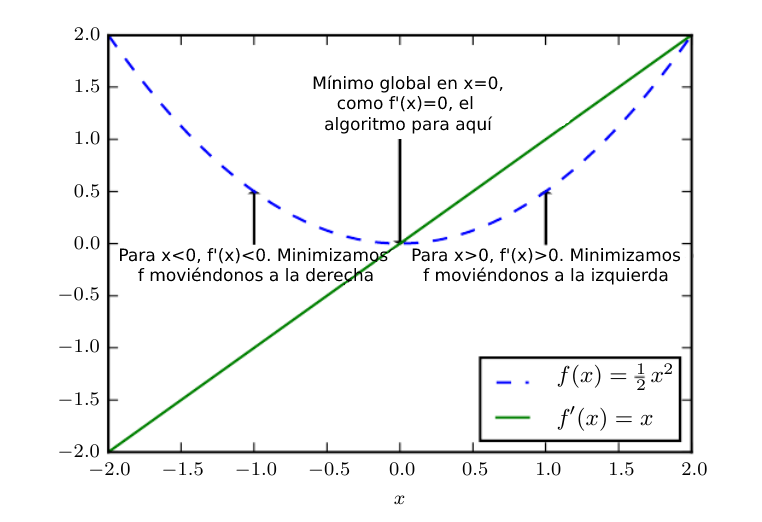
\includegraphics[width=0.75\linewidth]{Plantilla_TFG_latex//imagenes//Mat//1.intro/1.1GDMatIntroGoodFellowBook.png}
    \caption{Esquematización de la estrategia de descenso del gradiente en un modelo con un solo parámetro x. El eje horizontal representa los valores que toma éste y el vertical representa el error del modelo en función de x. Imagen obtenida y traducida del libro \cite{GoodFellowBook}}
    \label{fig:1.GD}
\end{figure}



Dependiendo de la familia de modelos que usemos podremos utilizar una estrategia de aprendizaje distinta, como el caso del \textit{Perceptron} y su \textit{Perceptron Learning Algorithm} \cite{patternrecog}. En otros casos como la regresión lineal se usa la estrategia de descenso de gradiente pero el gradiente no tiene por qué calcularse a través de BP. Esto se debe a que en este caso se puede obtener eficientemente a través de librerías matemáticas como \textit{numpy} \footnote{https://numpy.org/} en el caso del lenguaje \textit{python} \footnote{https://es.python.org/}, ya que esta familia de modelos conllevan menos costo computacional en sus cálculos principalmente debido al escaso número de parámetros en comparación con los de aprendizaje profundo. Para éste sí que es necesario el uso de BP en el caso de que elijamos entrenar mediante gradiente descendente, ya que aunque existen otras alternativas como los métodos numéricos o algunas aproximaciones recientes , no consiguen igualar su rendimiento \cite{EffBackProp, GoodFellowBook, alternativabacknumerical, alternativabackprop1}.


Otra de las características de este algoritmo para el cálculo del gradiente es que los conceptos en los que se basa son simples: optimización, diferenciación, derivadas parciales y regla de la cadena. Lo cual lo convierte a priori en objeto de estudio accesible. En la práctica, los cálculos que se realizan en esta estrategia se implementan a través de la diferenciación automática, que es una técnica más general que extiende a BP y se usa para el cómputo de derivadas de funciones numéricas de una manera eficiente y precisa \cite{AutomaticDiff}.% Ésta aprovecha el hecho de que cada cálculo que se realiza en un ordenador queda reducido a una secuencia de operaciones aritméticas elementales (suma, resta, multiplicación...) y funciones elementales (exponencial, trigonométricas, ...) para aplicar de forma repetida la regla de la cadena a estos elementos básicos hasta poder obtener derivadas de orden arbitrario. 



\subsection{Motivación}

Tenemos pues que el aprendizaje profundo es el paradigma del aprendizaje automático que mejores resultados obtiene actualmente y más desarrollo e investigación está concentrando, y que basa el entrenamiento (una de las partes fundamentales que determinan el rendimiento del modelo, además de su arquitectura) de los modelos casi por completo en el algoritmo de descenso de gradiente, ya que es el que mejores resultados de generalización ofrece. Éste a su vez depende casi enteramente del algoritmo de BP para calcular el gradiente, ya que aunque existan otras alternativas no son realmente viables. Tanto es así que es muy común la confusión entre éste algoritmo y el de gradiente descentente, que se suelen tomar por la misma cosa. Queda así clara la importancia que tiene BP en el campo del aprendizaje profundo y por extensión también al aprendizaje automático. También conviene destacar la cantidad de veces que se utiliza ésta técnica durante el entrenamiento de un modelo. Cada vez que se actualizan los pesos debemos calcular el gradiente, y teniendo en cuenta la duración de los entrenamientos de los modelos más grandes (con mayor número de parámetros) este algoritmo puede ser usado miles de veces durante un entrenamiento.

Su eficiencia, escalabilidad y flexibilidad lo han convertido en la opción por defecto para el entrenamiento basado en gradiente descendente para modelos de aprendizaje profundo, sin embargo no hay que olvidar que no se trata de una tarea sencilla: la obtención de un mínimo global y la verificación, dado un punto, de que es un mínimo global, se trata de un problema NP-Completo generalmente \cite{NPHardProblem}, por lo que se buscan estrategias aproximadas capaces de obtener buenas soluciones en tiempos razonables. Uno de los problemas abiertos en el aprendizaje profundo y en el que influye directamente BP es la reducción computacional del entrenamiento: si se ajustan los pesos en un modelo con un número muy alto de parámetros y usando un conjunto de entrenamiento muy grande (que es una tendencia reciente en aprendizaje profundo), los recursos computacionales pueden resultar insuficientes incluso para las grandes compañías, pudiendo requerir de meses para el  entrenamiento. Por lo que se necesitan algoritmos más escalables y eficientes para afrontarlo \cite{Problem3_accel}.

Por ello resulta esencial, mientras no existan alternativas viables, poder ofrecer modificaciones a este algoritmo para mejorar sus cualidades. Atendiendo a la cantidad de uso y su extensión en el campo, una pequeña mejora tendría un alcance enorme. Sin embargo esta línea de investigación no es muy extensa ya que principalmente se buscan alternativas en lugar de mejoras, pudiendo deberse principalmente a que a priori puede parecer una técnica muy enrevesada y compleja. Veremos en el desarrollo de esta parte que esto no es cierto, y que los principios en los que se basa son muy simples. Es clave comprender su base teórica, funcionamiento e implementación práctica para poder proponer mejoras. 


\subsection{Objetivos}

El objetivo principal de esta parte es realizar una investigación sobre los algoritmos de descenso de gradiente y \textit{backpropagation}, proporcionando una visión detallada acerca de los mismos y su implementación. Para ello se divide este objetivo en varios:

\begin{enumerate}
    %\item Exposición de la importancia actual e histórica en el campo del aprendizaje automático y aprendizaje profundo, viendo su estrecha relación con el algoritmo de aprendizaje del gradiente descente.

    
    \item Definir de manera detallada la base teórica y funcionamiento del algoritmo de descenso de gradiente atendiendo a elementos clave como su convergencia. Enunciar y demostrar resultados teóricos sobre la convergencia y analizar los problemas de ésta.

    \item Explorar el uso de BP para el cálculo del gradiente, analizando su implementación a través de la diferenciación automática.

    %\item Analizar de modo teórico las principales variantes del algoritmo de descenso de gradiente. 

 %   \item Realizar una investigación y revisión teórica de las alternativas al cálculo de gradiente basadas en otras estrategias como los métodos numéricos, e inviabilidad de las mismas frente a BP.
\end{enumerate}





%

\section{Fundamentos previos}
A continuación se definirán los conceptos básicos necesarios con los que se trabajará durante el desarrollo de esta parte. Se tratarán los elementos necesarios que se usan en el algoritmo de gradiente descendente y BP. Se presenta únicamente el material estrictamente necesario para comprender el trabajo. Se ha usado para la elaboración de esta sección los apuntes en línea del profesor de la UGR Rafael Payá Albert en su curso de Análisis Matemático I \footnote{\url{https://www.ugr.es/~rpaya/docencia.htm\#Analisis}}.  Salvo otras especificaciones, el material de consulta para el desarrollo de esta parte matemática ha sido el curso en línea de Ciencias de Computación de la universidad Bristish Columbia \footnote{\url{https://www.cs.ubc.ca/~schmidtm/Courses/5XX-S22/}} y los libros Probabilistic Machine Learning \cite{murphy2022probabilistic} y Deep Learning \cite{GoodFellowBook}


\subsection{Cálculo diferencial}

A continuación se definirán los principales conceptos que se usarán durante el presente TFG. Los algoritmos de gradiente descendente y BP se basan principalmente en el cálculo diferencial, y el hecho de que no usen herramientas matemáticas demasiado complejas resulta precisamente una de sus virtudes, ya que gracias a la abstracción y a un diseño ingenioso consiguen obtener grandes resultados a partir de operaciones relativamente sencillas. Empezamos con los conceptos más elementales que subyacen durante todo el trabajo.

Tomaremos $X$ e $Y$ como dos espacios normados no triviales cualesquiera. Se fija una función $f:A \rightarrow Y$ donde $\varnothing \neq A\subseteq X$ y un punto $a \in A^{\circ}$

\begin{definicion}[Función diferenciable]
    $f$ es diferenciable en el punto $a$ si existe una aplicación lineal y continua $T \in L(X,Y)$ que verifica:

    $$\displaystyle \lim_{x \to a} \frac{\left\| f(x)-f(a)-T(x-a)\right\|}{\left\| x-a\right\|}=0$$
    
    Decimos que $f$ es diferenciable si es diferenciable en todo punto del interior de su dominio.
\end{definicion}


\begin{definicion}[Derivada parcial]
        Sea $f: \Omega \subset \mathbb{R}^n \rightarrow Y \subset \mathbb{R}^M$, con $\Omega$ un abierto, $f=(f_1, f_2, ..., f_M)$, $a \in \Omega$, $k \in I_n$. Entonces $f$ es parcialmente derivable con respecto a la $k$-ésima variable en $a$ si, y sólo si, lo es $f_j \forall j \in I_M$, en tal caso, 

        $$\frac{\partial f}{\partial x_k}(a) = \left ( \frac{\partial f_1}{\partial x_k}(a), ..., \frac{\partial f_M}{\partial x_k}(a) \right ) \in \mathbb{R}^M$$

        $f$ es parcialmente derivable en $a$ si, y sólo si, lo es respecto de todas sus variables
\end{definicion}


Definimos ahora los elementos clave del proceso: el vector gradiente y la matriz jacobiana. En el algoritmo de descenso de gradiente, lo que se pretende calcular tal como indica el nombre es el vector gradiente, ya que la función de error de los modelos siempre nos devuelve un escalar, es decir que la dimensión de la imagen es 1, y la dimensión de la entrada será el número de parámetros del modelo (número de elementos que tendrá el vector gradiente). Sin embargo las matrices jacobianas también juegan un papel fundamental ya que para calcular ese vector gradiente, el algoritmo de BP necesita de cálculos intermedios, que son las matrices jacobianas asociadas entradas y salidas de las capas ocultas (que tienen mayor dimensionalidad) con respecto a parte de los parámetros (los parámetros de esa capa). 

\begin{definicion}[Vector gradiente]
    Sea $f:\Omega \subset \mathbb{R}^N \rightarrow \mathbb{R}$ un campo escalar, con $\Omega$ un abierto y $a \in \Omega$ . Cuando $f$ es parcialmente derivable en $a$, el gradiente de $f$ en $a$ es el vector $\nabla f(a) \in \mathbb{R}^N$ dado por 
    $$\nabla f(a) = \left ( \frac{\partial f}{\partial x_1} (a), \frac{\partial f}{\partial x_2} (a), ..., \frac{\partial f}{\partial x_N} (a) \right )$$
\end{definicion}


Fijamos un abierto $\Omega \subset \mathbb{R}^N$
, y la función $f:\Omega \rightarrow \mathbb{R}^M$. Notamos por $f= \left ( f_1,f_2,..., f_M \right )$ indicando las $M$ componentes de $f$ que son campos escalares definidos en $\Omega$, siendo $f_j=\pi _j \circ f$.

\begin{definicion}[Matriz jacobiana]
    Si $f$ es diferenciable en $ x \in \Omega$, la matriz jacobiana es la matriz de la aplicación lineal $Df \in L \left ( \mathbb{R}^N, \mathbb{R}^M \right )$ y se escribe como $J_f$. Viene dada por:

    $$J_f(x)= \begin{pmatrix}
 \frac{\partial f_1}{\partial x_1} & \frac{\partial f_1}{\partial x_2} & \cdots & \frac{\partial f_1}{\partial x_N} \\
 \frac{\partial f_2}{\partial x_1} & \frac{\partial f_2}{\partial x_2} & \cdots & \frac{\partial f_2}{\partial x_N} \\
 \vdots & \vdots & \ddots & \vdots \\
 \frac{\partial f_M}{\partial x_1} & \frac{\partial f_M}{\partial x_2} & \cdots & \frac{\partial f_M}{\partial x_N} \\
\end{pmatrix}= \begin{pmatrix}
 \nabla f_1(x)^T\\
 \vdots \\
 \nabla f_M(x)^T \\
\end{pmatrix}=
\begin{pmatrix}
     \frac{\partial f}{\partial x_1} \cdots \frac{\partial f}{\partial x_N}
\end{pmatrix}$$
\end{definicion}


Se presenta a continuación una de las reglas más útiles para el cálculo de diferenciales, que afirma que la composición de aplicaciones preserva la diferenciabilidad. Será parte clave en el desarrollo próximo ya que a los modelos de aprendizaje automático basados en capas podemos describirlos como una función que se descompone en una función por cada capa, por tanto será una herramienta que usaremos continuamente para calcular estas matrices jacobianas y gradientes.

\begin{teorema}[Regla de la cadena]
    Sean $X, Y, Z $ espacios normados, $\Omega$ un abierto no vacío de $X$ y $U$ lo es de $Y$, y las funciones $f:\Omega \rightarrow U$ y $g:U \rightarrow Z$. Entonces si $f$ es diferenciable en $a \in \Omega$ y g es diferenciable en $b=f(a)$ se tiene que $f \circ f$ es diferenciable en $a$ con

    $$D(g \circ f)(a) = Dg(b) \circ Df(a) = Dg(f(a)) \circ f(a)$$

    \raggedright{Si $f \in D(\Omega, Y)$ y  $g \in D(U,Z)$, entonces $g \circ f \in D(\Omega, Z)$.}
    
\end{teorema}


En ocasiones en algunos modelos tenemos que lidiar con funciones que no son diferenciables en un punto, y para poder manejarlas extenderemos el concepto de diferenciabilidad a lo que llamaremos subdiferenciabilidad. Esto se expondrá más adelante ya que son conceptos que no se han explorado a lo largo del grado de matemáticas.



\begin{comment} %Esto creo que no lo uso
	\begin{definicion}[Función continuamente diferenciable]
	    Si una función $f$ parcialmente derivable tiene todas sus derivadas parciales continuas, decimos que la función $f$ es continuamente diferenciable. Decimos que es de clase $C^1$.
	\end{definicion}
\end{comment}


\begin{comment}
    
	
	\begin{definicion}[Conjunto conexo]
	    Un espacio métrico $E$ es convexo si no puede ser expresado como unión de dos subconjuntos abiertos, no vacíos y disjuntos. Podemos formularlo de la siguiente manera:
	
	    $$U=U^{\circ}, V=V^{\circ}, U \cup V = E, U \cap V = \emptyset \Rightarrow U=\emptyset ó V=\emptyset$$
	\end{definicion}
	
	Caracterizamos de manera sencilla un espacio conexo:
	
	\begin{itemize}
	    \item \textit{Un espacio métrico $E$ es conexo si, y sólo si, para cualesquiera dos puntos $x,y \in E$ existe un conjunto conexo $C \subset E$, tal que $x,y \in C$}
	\end{itemize}
	
	Podemos decir de esta manera que un espacio métrico $E$ es conexo cuando cualquiera dos puntos de $E$ están conectados, es decir, existe un subconjunto conexo de E que los contiene.

\end{comment}




\begin{comment}
	
	\begin{definicion}[Función estrictamente convexa]
	    Sea $E \subset \mathbb{R}^n$ un conjunto convexo no vacío y sea $f:E \rightarrow \mathbb{R}$, $f$ es una función convexa en $E$ si, y solo si:
	
	    $$f(tx + (1-t)y) < tf(x) + (1-t) f(y), \quad \forall t \in ]0,1[, \forall x,y \in E, x \neq y$$
	\end{definicion}
	
	\begin{definicion}[Función fuertemente convexa]
	    Sea $E \subset \mathbb{R}^n$ un conjunto convexo no vacío y sea $f:E \rightarrow \mathbb{R}$, $f$ es una función fuertemente convexa en $E$ con módulo $c>0$ si :
	
	    $$f(tx + (1-t)y) \leq tf(x) + (1-t) f(y) - \frac{c}{2}t(1-t)\|x-y\|^2, \quad \forall t \in [0,1], \forall x,y \in E$$
	\end{definicion}
\end{comment}


\subsection{Lipschitz}

El último concepto, que también resulta de gran importancia en los resultados teóricos sobre la convergencia del gradiente descendente, es el de la condición de lipschitz, en concreto aplicada al gradiente

\begin{definicion}[Función Lipschitziana]
    Si $E$ y $F$ son espacios normados, una función $f:E \rightarrow F$ es lipschitziana si existe una constante $M \in \mathbb{R}_0^+$ que verifica:
    $$ \| f(x) - f(y) \| \leq M \| x - y \| \qquad \forall x,y \in E$$
\end{definicion}

Decimos que la función $f$ tiene gradiente lipschitziano si la condición anterior se aplica a su gradiente.

$$\| \nabla f(x) - \nabla f(y) \| \leq M \| x - y \| \qquad \forall x,y \in E $$


La mínima constante $M_0=L$ que verifica las desigualdades anterior es denominada la constante de Lipschitz de $f$ y viene definida por 

$$L=sup \left \{ \frac{\|f(x)-f(y)\|}{\|x - y \|} : x,y \in E, x \neq y \right \}$$

La definición nos dice de manera intuitiva que el gradiente de la función no puede cambiar a una velocidad arbitraria. %Esto es una suposición que podemos realizar de manera general para la función de error de la gran mayoría de modelos de aprendizaje automático. 

Para las funciones de clase $C^2$, es decir las que son diferenciables al menos dos veces con su derivada continua, una equivalencia a que el gradiente de $f$ sea lipschitziano es que $\nabla^2 f(x) \preceq LI \quad \forall x \in E$. Es decir que los valores propios de la matriz Hessiana están mayorados por $L$. Esta equivalencia la usaremos luego en la demostración \ref{proof:gdconvex}

\begin{comment}
	
	\subsection{Convergencia}
	%https://esfm.egormaximenko.com/numerical_methods/convergence_order_es.pdf
	
	Sea ${a_n}$ una sucesión que converge a b, con $a_n \neq b \quad \forall n \in \mathbb{N}$.
	
	\begin{definicion}[Orden de convergencia]
	    Sean $\alpha>0$ y $\lambda>0$, si se verifica
	
	    $$\lim_{n\rightarrow \infty} \frac{|a_{n+1}-b|}{|a_n - b|^{\alpha}} = \lambda$$
	
	    Entonces decimos que la sucesión ${a_n}$ converge a b con orden de convergencia $\alpha$ y constante de error asintótica $\lambda$.
	\end{definicion}

\end{comment}


%\section{Gradiente Descendente}

Se trata de un algoritmo de aprendizaje iterativo clásico, basado en el método de optimización para funciones lineales de Cauchy. Haskell Curry lo estudió por primera vez para optimización no lineal en 1944 \cite{Curry1944GDNoLin}, siendo ampliamente usado a partir de las décadas de los 1950-1960. Actualmente se trata de la estrategia de entrenamiento de modelos más ampliamente usada, especialmente en los modelos de aprendizaje profundo, siendo la estrategia que mejores resultados consigue en cuanto a capacidad de generalización de los modelos y eficiencia computacional gracias a su aplicación a través del algoritmo de BP. Sin embargo a nivel práctico no se usa en su versión original, sino que a lo largo del tiempo han ido surgiendo numerosas modificaciones con el objetivo de mejorar el algoritmo en diversos ámbitos: aumento de la estabilidad y la velocidad de convergencia, reducción computacional del entrenamiento, capacidad de evitar mínimos locales, etc. Estos métodos modificados del original se conocen como optimizadores. La literatura en este sentido es extensa, y aunque es bastante claro que el gradiente descendente sigue siendo la mejor estrategia de optimización de parámetros de un modelo de forma general, la elección del algoritmo de optimización concreto y de su ajuste depende del problema concreto que estemos tratando y generalmente se realiza de manera experimental. 

Debemos ver que el entrenamiento de los modelos, en su gran mayoría, está intrínsecamente ligado a la optimización, específicamente a la minimización de la función de coste $C$. Este no es un problema sencillo, y como se ha mencionado antes se trata de un problema NP-Completo, por tanto de existir algoritmos exactos estos requieren demasiado coste computacional como para utilizarlos en la práctica, por lo que se buscan estrategias aproximadas como el descenso de gradiente para obtener buenas soluciones en un tiempo asequible. 

Otros factores a tener en cuenta son la necesidad de escapar de óptimos locales, aún no conociendo de manera explícita la función de error; y la importancia de la generalización: no es  importante únicamente obtener un error bajo sino que ese error se mantenga cuando usamos datos de entrada nuevos, siendo preferible aumentar un poco el error en el entrenamiento si con ello conseguimos mejorar la generalización del modelo.


\subsection{Gradiente descendente de Cauchy}

Procedemos a describir el método original de descenso de gradiente, propuesto en 1847 por Augustin-Louis Cauchy \cite{CauchyGD}. Es una versión más primitiva y limitada que sus desarrollos posteriores pero que nos permite obtener de forma más sencilla una visión de su funcionamiento. 

Definimos $f:\mathbb{R}^N \rightarrow \mathbb{R}$ una función que es continua en todas sus variables\footnote{Realmente solo necesitamos que sean continuas en el intervalo concreto en el que se moverán.} y las cuales no toman valores negativos. Notamos a las variables por $x= \left ( x_1,...,x_N \right ) \in \mathbb{R}^N$. Si queremos encontrar los valores de $x_1,...,x_N$ que verifican $f(x_1,...,x_N)=0$, bastará con hacer decrecer indefinidamente los valores de la función $f$ hasta que sean muy cercanos a $0$. 

Fijamos ahora unos valores concretos $x_0 \in \mathbb{R}^N$, $u=f(x_0)$, $Du= \left ( D_{x_1}u, D_{x_2}u, ..., D_{x_N}u \right )$ y $\epsilon >0$ con $\epsilon \in \mathbb{R}^N$. Si tomamos $x_0'=x_0+\epsilon$ tendremos:
$$f(x_0')= f(x_0 + \epsilon) = u + \epsilon Du$$

Sea ahora $\eta >0$, tomando $\epsilon= - \eta Du$ con la fórmula anterior tenemos: 

$$f(x_0') = f(x_0 + \epsilon) = u - \eta \sum_{i=1}^{N}(D_{x_i}u)^2$$

Por tanto hemos obtenido un decremento en el valor de la función $f$ modificando los valores de sus variables en sentido contrario al gradiente, para $\eta$ suficientemente pequeño. Si aumentamos el valor de $\eta$ entonces el valor de la función decrecerá hasta cero o en caso contrario hasta alcanzar un mínimo. 




\subsection{Gradiente descendente en el entrenamiento de modelos}

En el caso del aprendizaje de modelos la función que debemos minimizar es la función de coste $C$, que efectivamente es continua por ser composición de funciones continuas, como se verá más adelante. Esta función no toma valores negativos. Como no podemos realizar un cálculo continuo para comprobar con qué valores de $\eta$ la función decrece, lo hacemos de manera iterativa, y a este $\eta$ lo llamamos ratio de aprendizaje o más comúnmente \textit{learning rate}. 

En el proceso de entrenamiento de un modelo lo que hacemos es aplicar la idea anterior de manera iterativa en lugar de encontrar un $\eta$ que minimice en un paso, para ir moviéndonos a puntos de menor valor de la función de coste. Si $C(W)$ es la función de coste del modelo y $W$ representa los parámetros del modelo, entonces la regla de actualización iterativa del descenso del gradiente es la siguiente:

\begin{equation}\label{eq:GD}
W_{t+1}=W_t - \eta \nabla C(W)
\end{equation}

En su descripción original, el gradiente se calcula usando todos los datos de entrenamiento, pero en versiones posteriores se propone dividir el conjunto de entrenamiento en varios subconjuntos disjuntos, denominados lotes. Cada vez que se calcula el gradiente se actualizan los pesos, y denominamos a esto una iteración. Cada vez que se usan todos los datos de entrenamiento para calcular el gradiente, ya sea tras una sola iteración usando todo el conjunto de entrenamiento o varias si dividimos en lotes, lo denominamos época.



\subsubsection{Estrategias de gradiente descendente} \label{sec:estrategias}

En base a los lotes en que dividamos el conjunto de entrenamiento tenemos varios tipos de gradiente descendente \cite{GoodFellowBook}.

\begin{itemize}
    \item \textbf{Batch Gradient Descent} (BGD): tenemos un único lote, cada iteración se corresponde con una época. Calculamos el gradiente usando todo el conjunto de entrenamiento. Esto ofrece un comportamiento mejor estudiado a nivel teórico, con más resultados demostrados; pero aumenta mucho el coste computacional del entrenamiento hasta el punto que lo vuelve demasiado lento para ser usado en la práctica.

    \item \textbf{Stochastic Gradient Descent} (SGD): Actualiza los pesos calculando el gradiente con sólo un elemento del conjunto de entrenamiento. Cada época tiene tantas iteraciones como número de elementos haya en el conjunto de entrenamiento. Esta estrategia introduce ruido en el entrenamiento ya que el gradiente se calcula de una manera aproximada, aunque esto tiene un efecto positivo ya que al provocar más irregularidad en la trayectoria de convergencia se puedan escapar mínimos locales. Además es más eficiente computacionalmente que el anterior y converge más rápido en la práctica.

    \item \textbf{Mini-Batch Gradient Descent} (MBGD): Se divide el conjunto de entrenamiento en M lotes de tamaño fijo, y se calcula el gradiente con cada lote, por lo que habrá M iteraciones en cada época. Se consigue una aproximación del gradiente con menos error al usar más datos para su cálculo y además se siguen manteniendo las propiedades que veíamos en la anterior estrategia. Es más eficiente que la anterior al conllevar menos actualizaciones de pesos. Es practicamente la única estrategia utilizada en la realidad ya que ofrece la mayor eficiencia computacional, estabilidad y rapidez en la convergencia.
\end{itemize}

Aunque la política para computar el gradiente sea distinta en estos 3 tipos, los englobaremos dentro de lo que denominaremos el algoritmo de gradiente descendente original, ya que como veremos más adelante, existen varias modificaciones del algoritmo que aportan mejoras a través de modificar la regla de actualización de los pesos y no solo la cantidad de datos con la que se aproxima el gradiente.

\subsubsection{\textit{Learning rate}}

El elemento $\eta$ que observamos en la ecuación \ref{eq:GD} del gradiente descendente se denomina \textit{learning rate} y lo usamos para controlar la convergencia reduciendo el efecto de la magnitud del gradiente en la actualización de los parámetros. Este valor es positivo y situado en la práctica alrededor de 0.01 y 0.001 usualmente, aunque para su elección conviene realizar un análisis teórico previo o realizar pruebas prácticas (mucho más común) para elegir un valor adecuado. Este tipo de parámetros, que no son parte del modelo sino del algoritmo de aprendizaje, se denominan hiperparámetros. Dependiendo del tipo de algoritmo o modifiación del mismo que usemos habrá diferentes hiperparámetros, siendo el \textit{learning rate} el más importante de manera general, ya que de su valor dependerá la convergencia del algoritmo, pudiendo hacer que converja demasiado lento o que directamente diverja, como podemos observar en la figura \ref{fig:lr} o en resultados sobre la convergencia en la sección \ref{sec:convergencia}.

En cuanto a la selección de los hiperparámetros, no se enfoca como un problema donde se busque el óptimo de estos valores ya que la mayoría no son tan decisivos en la convergencia como el \textit{learning rate}, y se ofrecen valores teóricos en sus papers de presentación que funcionan bien en casos generales. Si bien la convergencia es sensible a los valores iniciales de estos hiperparámetros que se tratan de optimizar a nivel experimental a través del ensayo y error, aunque no se dedican excesivos recursos computacionales a esta búsqueda, invirtiéndose por el contrario en el entrenamiento.



\begin{figure}
    \centering
    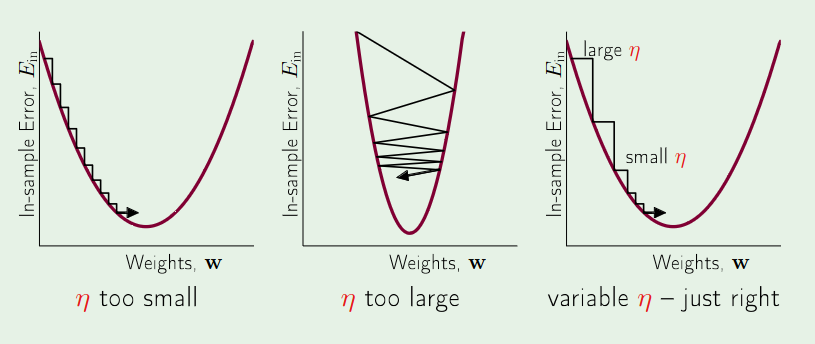
\includegraphics[width=0.5\linewidth]{Plantilla_TFG_latex//imagenes//Mat//GD/lr.png}
    \caption{Visualización de cómo afecta el \textit{learning rate} según su adecuación al problema. Imagen obtenida del curso de Caltech \footnote{https://home.work.caltech.edu/slides/slides09.pdf}, tema 9 diapositiva 21}
    \label{fig:lr}
\end{figure}

Una táctica habitual es usar una política de \textit{learning rate} que decrezca conforme avanza el entrenamiento, de manera que el algoritmo avance con pasos más grandes cuando aún está lejos del óptimo, con un objetivo explorador, y con pasos más pequeños cuando se va acercando, con un objetivo explotador, procurando una convergencia más estable. \cite{GoodFellowBook}. Otro enfoque común es también tener un vector de \textit{learning rate} en lugar de un solo escalar, teniendo un valor para cada peso del modelo. 





\subsection{Subgradientes} \label{sec:subgrad}

Con el objetivo central de calcular el gradiente es lógico pensar que necesitamos ciertas condiciones de diferenciabilidad, aunque sean mínimas, para poder calcular el gradiente que necesitamos. Podemos pensar en un modelo como una composición de la suma y producto de operaciones lineales con operaciones no lineales (funciones de activación), y componiendo ésta con la función de coste del modelo obtendríamos la función $f: X \times \Omega \times Y \rightarrow \mathbb{R^+}$, que recibe los pesos del modelo, los datos de entrada y sus etiquetas correctas para proporcionar el error del modelo. Esta es la función que necesitaríamos que fuera diferenciable. Las operaciones lineales preservan la diferenciabilidad, y la composición de funciones diferenciables es diferenciable por lo que si la función de pérdida y las funciones de activación son diferenciables, no tendremos ningún problema a la hora de calcular el gradiente.

\begin{itemize}
    \item \textbf{ECM:} $\frac{1}{N} \sum_{i=1}^N \left (y_i - \hat{y} \right ) ^2$ 

    \item \textbf{\textit{CrossEntropyLoss}:} $  - \sum_c \hat{y_c} log(\frac{e^{y_c}}{\sum_{c'=1}^C e^{y_{c'}}})$
\end{itemize}

Las funciones de coste son diferenciables de manera general, y las más comunes son por ejemplo el error cuadrático medio para problemas de regresión y \textit{CrossEntropyLoss} para problemas de clasificación. Donde $N$ es el número de datos, $\hat{y}_i$ es el valor real del dato $i$, que en ECM será un escalar, y en clasificación binaria será 0 ó 1; $y_c$ es el valor predicho por el modelo, $\hat{y}_{c}$ es la etiqueta real de la clase $c$, que valdrá 1 en caso de que el dato pertenece a la clase $c$ y 0 en caso contrario; y $y_{c}$ es el predicho por el modelo. 


Hasta el año 2010, las funciones de activación más comunes para las capas ocultas eran la función sigmoide y la tangente hiperbólica. Estas funciones son diferenciables por lo que su uso no suponía ningún problema. Sobre ese año empezaron a popularizarse las funciones de activación ReLU (Rectified Linear Unit), gracias a su simplicidad, reducción de coste computacional y su aparición en modelos ganadores de competiciones de ImageNet como AlexNet en 2012. Desde entonces esta función, junto a algunas de sus variantes que aparecen en la figura \ref{fig:3.ReLU} son ampliamente usadas y con buenos resultados. Sin embargo salta a la vista que esta función no es diferenciable.


\begin{figure}
    \centering
    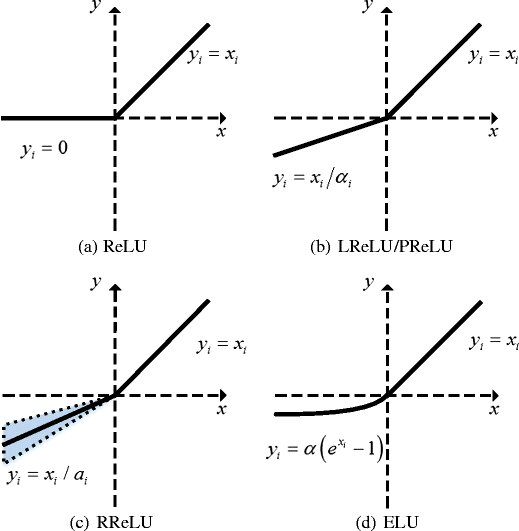
\includegraphics[width=0.5\linewidth]{3ReLU&oth.jpg}
    \caption{Función ReLU y algunas de sus variantes más usadas como funciones de activación.\footnote{https://www.researchgate.net/publication/319438080\_A\_novel\_softplus\_linear\_unit\_for\_deep\_convolutional\_neural\_networks}}
    \label{fig:3.ReLU}
\end{figure}



Vamos a presentar entonces el concepto de subgradiente junto con algunas de sus propiedades, obtenidas de \cite{convexSubgrad}, para ver que será una extensión del gradiente que nos permitirá usar el método de gradiente descendente con funciones que no sean diferenciables en algunos puntos pero que sí sean subdiferenciables.

\begin{definicion}[Subgradiente]
     Sea $A \subset \mathbb{R}^n$ y $f:A \rightarrow \mathbb{R}$, $g \in \mathbb{R}^n$ es un subgradiente de $f$ en $a \in A$ si $\forall y \in A$ se tiene:

    $$f(a)-f(y) \leq g^T(a-y)$$
    El conjunto de los subgradientes de $f$ en x se denota por $\partial f(a)$. Si existe el subgradiente de $f$ en a, decimos que $f$ es subdiferenciable en $a$.
\end{definicion}

Tenemos que comprobar que el subgradiente extiende al gradiente, es decir, que cuando existe gradiente entonces existe el subgradiente y coincide con él, y además hay funciones que no tienen el gradiente pero sí subgradiente. Vamos a definir lo que es un conjunto convexo, ya que resulta elemental tanto en esta sección como en la siguiente y usaremos este concepto para desarrollar otros a partir de él.


\begin{definicion}[Conjunto convexo]
    Un subconjunto $E$ de un espacio vectorial $X$ es convexo cuando, para cualesquiera dos puntos de $E$, el segmento que los une está contenido en $E$:

    $$x,y \in E \Rightarrow \left \{ (1-t)x + ty : t\in [0,1] \right \} \subset E$$
\end{definicion}

\begin{proposicion}[Existencia de subgradientes]
\label{prop:subgrad}
    Sea $A \subset \mathbb{R}^n$ un conjunto convexo y $f:A \rightarrow \mathbb{R}$. Si $\forall a \in A, \partial f(x) \neq \emptyset$ entonces $f$ es una función convexa. Recíprocamente, si $f$ es convexa $\forall x \in int(A)$ entonces se tiene que $\partial f(x) \neq \emptyset$. Además si $f$ es convexa y diferenciable en x se verifica que $\nabla f(x) \in \partial f(x)$.
\end{proposicion}

Para demostrar esta proposición, primero vamos a necesitar de un teorema, en el ámbito de la convexidad:

\begin{teorema}[Teorema del Hiperplano de apoyo]
    Sea $X \subset \mathbb{R}^n$ un conjunto convexo y $x_0$ un puntro de la frontera de $X$. Entonces, $\exists w \in \mathbb{R}^n, w \neq 0$ tal que
    $$\forall x \in X, \quad w^Tx \geq w^T x_0$$
\end{teorema}

\textbf{\textit{Demostración.}}
Para la primera implicación, queremos probar que $f((1-t)x+ty) \leq (1-x)f(x)+tf(y) \forall x,y \in X, \quad t \in [0,1]$, es decir, que $f$ es convexa. Partiendo de que $\forall x \in X, \quad \partial f(x) \neq \emptyset $, tomando cualquier $g \in \partial(z), \quad z \in X$ tenemos por la definición de subgradiente:

$$f(z) - f(x) \leq g^T(z-x),$$
$$f(z) - f(y) \leq g^T(z-y),$$

Para $x,y \in X$. Tomamos $z=(1-t)x + ty$ y sustituimos:
$$f((1-t)x + ty) - f(x) \leq g^T(((1-t)x + ty)-x),$$
$$f((1-t)x + ty) + g^T(x - ((1-t)x-ty) \leq f(x),$$
$$f((1-t)x + ty) + g^T(t(x-y) \leq f(x),$$

\begin{equation}\label{proof1:f(x)}
    f((1-t)x + ty) + tg^T(x-y) \leq f(x)
\end{equation}

Desarrollando en la otra desigualdad de manera análoga obtenemos

\begin{equation}\label{proof1:f(y)}
    f((1-t)x + ty) + (1-t)g^T(y-x)) \leq f(y)
\end{equation}

Ahora multiplicamos la desigualdad \ref{proof1:f(x)} por $(1-t)$ y la \ref{proof1:f(y)} por $t$, y de su suma obtenemos:

\begin{gather*}
(1-t)f(x) + tf(y) \geq \\
 (1-t)f((1-t)x+ty) + t(1-t)g^T(x-y) + tf((1-t)x+ty) + t(1-t)g^T(y-x) \\
 = f((1-t)x + ty) + t(1-t) g^T(x-y) + t(1-t)g^T(y-x)
\end{gather*}

Como se tiene que $g^T(x-y) + g^T(y-x)=0$, entonces tenemos que $(1-t)f(x) + tf(y) \geq f((1-t)x + ty), \quad \forall x,y \in X, \quad t \in [0,1]$. Por tanto $f$ es convexa, como queríamos probar.

Ahora vamos a probar que $f$ tiene algún subgradiente en $int(X)$. Definimos el epigrafo de una función $f$ como $epi(f)=\left \{ (x,t) \in X \times \mathbb{R} : t \geq f(x) \right \}$. Es obvio que f es convexa si y sólo si su epigrafo es un conjunto convexo. Vamos a aprovechar esta propidad y vamos a construir un subgradiente usando un hiperplano de apoyo al epigrafo de la función. Sea $x \in X$, claramente $(x, f(x)) \in \partial epi(f)$, y $epi(f)$ es un conjunto convexo por ser $f$ convexa. Entonces usando el Teorema del Hiperplano de Apoyo, existe $(a,b) \in \mathbb{R}^n \times \mathbb{R}$ tal que

\begin{equation}\label{proof1:epi}
    a^Tx + bf(x) \geq a^Ty + bt, \forall (y,t) \in epi(f)
\end{equation}

Reordenando tenemos

$$b(f(x)-t) \geq a^Ty - a^Tx$$

Como $t \in [f(x), + \infty [$, para que se mantenga la igualdad incluso cuando $t \rightarrow \infty$, necesitamos que $b\leq 0$. Ahora vamos a asumir que $x \in int(X)$. Entonces tomamos $\epsilon > 0$, verificando que $y=x+\epsilon a \in X$, lo que implica que $b\neq 0$, ya que si $b=0$ entonces necesariamente $a=0$. Reescribiendo \ref{proof1:epi} con $t=f(y)$ obtenemos

$$f(x) - f(y) \leq \frac{1}{|b|} a^T (x-y)$$

Por tanto $\frac{a}{|b|} \in \partial f(x)$, lo que demuestra la segunda parte de la proposición.

Para la última parte, sea $f$ una función convexa y diferenciable. Entonces por definición para $t \in [0,1]$ y $x,y \in X$

$$tf(y) + (1-t)f(x) \geq f((1-t)x + ty)$$

$$f(y) \geq \frac{f((1-t)x + ty) - (1-t)f(x)}{t}$$

$$= f(x) + \frac{f(x + t(y-x)) - f(x)}{t}$$

$$ \xrightarrow[t \rightarrow 0]{} \quad f(x) + \nabla f(x)^T (y-x)$$

Lo que demuestra que $\nabla f(x) \in \partial f(x)$


\begin{flushright}
    $\square$
\end{flushright} 




Necesitamos también un comportamiento similar al de las funciones diferenciables, en particular necesitamos que las funciones subdiferenciables se preserven a través de las operaciones de suma, multiplicación por escalares y composición.

\begin{enumerate}

	\item \textbf{Multiplicación escalar no negativa}: $\partial (af) = a \cdot \partial f , a\geq0$
	
	\item \textbf{Suma}: $\partial (f_1+f_2) = \partial f_1 + \partial f_2$
	
	\item \textbf{Composición afín}: Si $g(x)=f(Ax + b) \Rightarrow \partial g(x)= A^T \partial f(Ax+b)$
	
	%\item \textbf{Máximo finito}: Si $f(x) = max_{i=1,...,n} f_i(x)$ entonces
	 %$$\partial f(x) = conv \left ( \underset{i: f_i(x)=f(x)}{\cup} \partial f_i(x) \right )$$
	
	%\item \textbf{Máximo general}: Si $f(x) = max_{s  \in S} f_s(x)$ entonces 
	%$$  \overline{\left \{  conv \left ( \underset{s:f_s(x)=f(x)}{\cup} \partial f_s(x) \right )    \right \}  \subseteq \partial f(x)}$$

\end{enumerate}

Tenemos entonces que el subgradiente es una extensión del gradiente en aquellos puntos que no son diferenciables. Por ello podríamos decir que existe el método de descenso de subgradiente, que permite usar funciones que no son diferenciables en todos los puntos, y que se usa de manera implícita en el momento en el que en un modelo se usan funciones ReLU, por ejemplo. Conviene destacar esta diferencia para no perder la rigurosidad, aunque solo sea una formalidad, ya que realmente no se hacen diferencias entre uno y otro método, así que nos seguiremos refiriendo al método de descenso de gradiente aunque estemos trabajando con subgradientes. En \cite{ReLuat0} se analiza la elección del valor que toma el subgradiente en el punto $x=0$ y se ve su influencia, que no es poca, en la ejecución del algoritmo, y se concluye que el valor 0 es el que ofrece mejor robustez de manera general.

\begin{ejemplo}[Subgradiente de la función ReLU]\label{ej:RELUsub}
     La función ReLU es continua en todo el dominio y diferenciable en $]-\infty,0[ \cup ]0,\infty[$. Su subgradiente es el siguiente:

    $$ \nabla ReLU(x)=\left\{\begin{matrix}
1, \quad si \quad x \in ]0,\infty[ \\
c \in [0,1] \quad si \quad x=0\\
0 \quad si \quad x \in ]-\infty,0[
\end{matrix}\right.$$
\end{ejemplo}




\subsection{Convergencia} \label{sec:convergencia}

La convergencia es un factor crucial en el algoritmo de gradiente descendente. Al tratarse de un algoritmo de optimización iterativo, iremos buscando el mínimo global de la función de coste en varios pasos, o en su defecto un mínimo local que nos ofrezca una solución subóptima. El algoritmo se mueve hacia puntos de menor gradiente por lo que convergerá a puntos donde el gradiente sea 0. Un factor clave para la convergencia será el hecho de que la función de pérdida sea o no una función convexa.




\begin{definicion}[Función convexa]
    Sea $E \subset \mathbb{R}^n$ un conjunto convexo no vacío y sea $f:E \rightarrow \mathbb{R}$, $f$ es una función convexa en $E$ si, y solo si:

    $$f(tx + (1-t)y) \leq tf(x) + (1-t) f(y), \quad \forall t \in [0,1], \forall x,y \in E$$
\end{definicion}


En caso de que la función de coste sea convexa sólo existirá un mínimo y será global, por lo que no tenemos que preocuparnos de si el algoritmo se queda estancado en un mínimo local, ya que si converge tenemos la solución óptima. Además en este caso el análisis de la convergencia resulta mucho más sencillo, y por eso encontramos más resultados teóricos y más fuertes que en el caso contrario. Desgraciadamente la situación normal es que la función de coste no sea convexa, y de hecho comprobar que una función sea convexa se trata de un problema NP-Hard \cite{Ahmadi_2011_NP_Convex}, por lo que en la práctia normalmente no realizamos el análisis teórico de la función y la convergencia previo al entrenamiento del modelo. En caso que no sea convexa, podemos converger hacia un punto crítico que no sea un mínimo global, con lo cual el algoritmo parará y puede que hallamos llegado a una solución que aunque sea subóptima no sea lo suficientemente buena.



\subsubsection{Resultados teóricos para la convergencia del gradiente descendente}

Los desarrollos teóricos sobre la convergencia del algoritmo de descenso del gradiente son muchos y variados. Los principales inconvenientes para el desarrollo de un marco teórico que sea útil en la práctica son:

\begin{itemize}

    \item No existen resultados generales que nos permitan conocer el comportamiento de la convergencia del algoritmo en el problema que estemos tratando con un coste asequible. Los resultados son muy específicos y dependen de la función de coste, el valor de los hiperparámetros y la versión del algoritmo de gradiente descendente que estemos utilizando.

    \item El estudio teórico de la función de coste es muy complejo y requiere tanto tiempo como recursos computacionales. Por lo tanto la tendencia a nivel experimental es invertir esos recursos en el entrenamiento, ya que ofrece mejores resultados en relación coste/beneficio de manera genérica que el estudio teórico de los elementos del algoritmo. Además es un procedimiento genérico aplicable en cualquier problema, por lo que resulta más sencillo.

    \item La mayoría de resultados teóricos aprovechables son basados en el gradiente descendente original (BGD), ya que cuando introducimos el ruido que genera la aproximación del cálculo del gradiente en sus variantes SGD y MBGD se complica el desarrollo teórico. Los resultados que aparecen a continuación son, a menos que se especifique lo contrario, resultados para BGD.
   
\end{itemize}


En el caso que la función de coste sea convexa tenemos un caso más sencillo de analizar, principalmente debido a la curvatura que tienen las funciones convexas y al hecho de que cualquier punto crítico será un mínimo global.

\begin{comment}
			
			\begin{proposicion}
			    Sea $f:\mathbb{R}^n \rightarrow \mathbb{R}$ una función de coste que es convexa con su gradiente $\nabla f$ Lipschitz continuo, con constante de Lipschitz $L>0$. Si el \textit{learning rate} $\eta$ se elige de manera que $0<\eta<\frac{2}{L}$, entonces el algoritmo de gradiente descendente converge a un punto $x_m$ que es mínimo global de la función $f$ \cite{murphy2022probabilistic}
			\end{proposicion}
			
			Esto nos asegura que seleccionando un \textit{learning rate} adecuado el algoritmo converge a un mínimo global, que es lo que buscamos. Como en la práctica es demasiado complejo encontrar la constante de Lipschitz, podemos seleccionar un valor suficientemente cercano a 0 para asegurarnos la convergencia y luego ir probando a aumentarlo poco a poco para obtener una velocidad de convergencia adecuada.
			
			Si tenemos una función de coste que, no solo es convexa, sino que es fuertemente convexa, entonces además de la convergencia a un mínimo global tenemos asegurada la velocidad de la convergencia de éste:
			
			
			\begin{proposicion}
			    Sea $f:\mathbb{R}^n \rightarrow \mathbb{R}$ una función de coste que es fuertemente convexa con su gradiente $\nabla f$ Lipschitz continuo, con constante de Lipschitz $L>0$. Entonces el algoritmo de gradiente descendente converge a un punto $x_m$ que es mínimo global de la función $f$, y además existe una constante $\rho \in [0,1]$ que verifica $\| x_k - x_m \| \leq \rho^k \| x_0 - x_m\|$. Es decir, la convergencia es lineal \cite{ConvexOp}.     
			\end{proposicion}
			
			Aunque el orden lineal no parezca demasiado bueno, en la anterior proposición ni siquiera la teníamos asegurada. En la práctica cuando usamos optimizadores generalmente conseguimos mayor orden de convergencia aunque no lo tenemos asegurado. Cabe recordar que, aunque usemos terminología referente a métodos iterativos, el gradiente descendente no es un método numérico.
			
			
			Ahora tenemos un resultado más general, no haciendo uso de funciones convexas. Este es el caso más común.

\end{comment}



\begin{teorema}[Convergencia para funciones convexas]\label{proof:gdconvex}
    Suponemos $f$ una función convexa y diferenciable, con su gradiente Lipschitz continuo con constante $L>0$, teniendo que $\| \nabla f(x) - \nabla f(y) \|_2 \leq L \|x-y\|_2 \quad \forall x, y$. Si ejecutamos el algoritmo de gradiente descendente $k$ iteraciones con un $\eta<1/L$ constante, el error disminuirá tras cada iteración, llegando a una solución $f^{(k)}$ que satisface la siguiente ecuación:

    $$f(x^{(k)})-f(x^*) \leq \frac{\|x^{(0)}-x^* \|^2_2}{2\eta k}$$

    Donde $x^*$ es el mínimo global de la función de error. 
\end{teorema}

\vspace{1cm}

\begin{flushleft}
   \textbf{\textit{Demostración.}}
\end{flushleft} 



En el teorema anterior $x \in \mathbb{R}^n$ son los pesos del modelo, y suponemos que el conjunto de datos con el que entrenamos es constante, por lo tanto el error del modelo, $f(x)$, sólo dependerá de los parámetros $x$.

Como $\nabla f$ es Lipschitz continuo con constante $L$ entonces $\nabla ^2 f(x) \preceq LI$, donde $I$ es la matriz identidad. Equivalentemente esto significa que $\nabla ^2 f(x) -LI$ es una matriz semidefinida negativa. Ahora hacemos un desarrollo cuadrático de $f$ alrededor de $f(x)$ para obtener:

\begin{gather*}
    f(y) \leq f(x) + \nabla f(x)^T (y-x) +\frac{1}{2}\nabla^2 f(x) \|y-x\|^2_2  \\
    \leq f(x) + \nabla f(x)^T(y-x) + \frac{1}{2}L \|y - x \|^2_2
\end{gather*}

Consideramos ahora $y$ como la actualización de los pesos del gradiente descendente, $y=x - \eta \nabla f(x)=x^+$. 


\begin{gather*}
    f(x^+) \leq f(x) + \nabla f(x)^T(x^+-x) + \frac{1}{2}L \|x^+ - x \|^2_2 \\
    = f(x) + \nabla f(x)^T(x - \eta \nabla f(x) -x) + \frac{1}{2}L \|x - \eta \nabla f(x) - x \|^2_2 \\
    = f(x) - \eta \nabla f(x)^T \nabla f(x) + \frac{1}{2} L \| \eta \nabla f(x) \|^2_2 \\
    = f(x) - \eta \| \nabla f(x) \|^2_2 + \frac{1}{2} L \eta^2 \| \nabla \|^2_2 \\
    = f(x) - (1- \frac{1}{2}L \eta) \eta \| \nabla f(x) \|^2_2
\end{gather*}

Usamos $\eta \leq \frac{1}{L}$ para ver que $-(1-\frac{1}{2}L \eta)= \frac{1}{2} L \eta - 1 \leq \frac{1}{2} L (\frac{1}{L}) - 1 = \frac{1}{2} - 1 = -\frac{1}{2}$, y sustituyendo esta expresión en la desigualdad anterior obtenemos 

\begin{equation}\label{eq:gdproof1}
	f(x^+) \leq f(x) - \frac{1}{2} \eta \| \nabla f(x) \|^2_2 
\end{equation}

Esta última desigualdad se traduce en que tras cada iteración del algoritmo del descenso de gradiente el valor del error del modelo es estrictamente decreciente, ya que el valor de $\frac{1}{2} \eta \| \nabla f(x) \|^2_2$ siempre es mayor que 0 a no ser que $\nabla f(x)=0$, en cuyo caso habremos encontrado el óptimo. 

Ahora vamos a acotar el valor del error en la siguiente iteración, $f(x^+)$, en términos del valor óptimo de error $f(x^*)$. Como $f$ es una función convexa se tiene

\begin{align*}
    f(x^*) \geq f(x) + \nabla f(x) ^T (x^* - x) \\
    f(x) \leq f(x^*) + \nabla f(x)^T (x-x^*)
\end{align*}

La segunda desigualdad se deduce de la primera de manera inmediata. Sustituyendo esa segunda desigualdad en \ref{eq:gdproof1} obtenemos

\begin{gather*}
    f(x^+) \leq f(x^*) + \nabla f(x)^T (x-x^*) - \frac{\eta}{2} \| \nabla f(x) \| ^2_2 \\ 
    f(x^+) - f(x^*) \leq  \frac{1}{2\eta}  \left ( 2 \eta \nabla f(x)^T (x-x^*) - \eta ^2 \| \nabla f(x) \| ^2_2 \right ) \\ 
    f(x^+) - f(x^*) \leq  \frac{1}{2\eta}  \left ( 2 \eta \nabla f(x)^T (x-x^*) - \eta ^2 \| \nabla f(x) \| ^2_2 - \| x - x^* \|^2_2 + \| x - x^* \|^2_2 \right )    
\end{gather*}

Como $  2 \eta \nabla f(x)^T (x-x^*) - \eta ^2 \| \nabla f(x) \| ^2_2 - \| x - x^* \|^2_2 = \| x - \eta \nabla f(x) - x^* \|^2_2 $, se tiene que

$$ f(x^+) - f(x^*) \leq  \frac{1}{2\eta}  \left ( \| x - x^+ \|^2_2 -  \| x - \eta \nabla f(x) - x^* \|^2_2 \right ) $$

Usamos ahora la definición de $x^+$ en esta última desigualdad

$$ f(x^+) - f(x^*) \leq  \frac{1}{2\eta}  \left ( \| x - x^+ \|^2_2 -  \| x^+ - x^* \|^2_2 \right ) $$

Hacemos la sumatoria sobre las $k$ primeras iteraciones y tenemos

\begin{gather*}
    \sum^k_{i=1} \left ( fx^{(i)} - f(x^*) \right ) \leq \sum^k_{i=1} \frac{1}{2\eta}  \left ( \| x^{(i-1)} - x^+ \|^2_2 -  \| x^{(i)} - x^* \|^2_2 \right ) \\ 
    \frac{1}{2\eta}  \left ( \| x^{(0)} - x^+ \|^2_2 -  \| x^{(k)} - x^* \|^2_2 \right ) \\ 
    \leq \frac{1}{2\eta}  \left ( \| x^{(i-1)} - x^+ \|^2_2 \right )  
\end{gather*}

El sumatorio de la derecha ha desaparecido ya que es una serie telescópica. Usando que $f$ decrece con cada iteración, e introduciendo la anterior desigualdad, finalmente llegamos a donde queríamos:

$$f(x^{(k)} - f(x^*) \leq \frac{1}{k} \sum ^k _{i=1} \left ( f(x^{(i)} - f(x^*) \right ) \leq \frac{\|x^{(0)}-x^* \|^2_2}{2\eta k} $$


\begin{flushright}
    $\square$
\end{flushright} 


Este teorema nos garantiza que bajo las condiciones supuestas el algoritmo del gradiente descendente converge y además lo hace con ratio de convergencia de $O(1/k)$. Es un resultado teórico muy fuerte que por desgracia no puede usarse en la práctica en la gran mayoría de casos: la constante de Lipschitz $L$ es computacionalmente costosa de calcular, por lo que se usan aproximaciones experimentales para el $\eta$, además en muy contadas ocasiones la función de error con la que trabajamos es convexa, y tampoco es sencilla de calcular por lo que directamente no se comprueba si lo es o no lo es, y directamente la suponemos no convexa. 

Podemos obtener un resultado mucho más práctico, ya que es para SGD y MBGD y además con condiciones más relajadas. Usando la teoría de algoritmos aproximados estocásticos, en concreto el teorema de Robbins-Siegmund tenemos que bajo las siguientes condiciones, cuando la función es convexa se tiene la convergencia casi segura al mínimo global y cuando no lo es hay convergencia casi segura a un punto crítico. Esto nos da un criterio sencillo para la convergencia, y que no depende de parámetros como la constante de Lipschitz que son complejos de computar.


\begin{proposicion}[Convergencia para SGD]
    Sea ${x_k}$ la secuencia generada por el algoritmo de SGD, sea $f$ la función de coste del modelo y sea $\eta_k$ el valor del \textit{learning rate} en la iteración $k$. Si la sucesión ${\eta_k}$ satisface $\sum_{k=1}^\infty \eta_k = \infty$ y también $\sum_{k=1}^\infty \eta_k ^2 < \infty$  entonces $\lim_{k\rightarrow\infty} \| \nabla f(x_k) \| =0$. Es decir, el algoritmo converge hacia un punto crítico de la función.% \cite{GoodFellowBook}.
\end{proposicion}

Aunque la complejidad de la demostración se escapa al alcance de este TFG, ya que sería necesario demasiadas definicones y resultados previos, en la página 33 de \cite{RobbinSiegmund} \footnote{El original 'A convergence theorem for non negative almost supermartingales and some applications' es de pago y no puedo acceder} podemos encontrar el enunciado y demostración del teorema de Robbins-Siegmund. En \cite{RobbinSiegmundtoSGD} podemos observar su uso para la demostracion de la convergencia de SGD. Hay que remarcar que, aunque la demostración de la convergencia se realiza en supuesto de función convexa a un mínimo global, se puede tomar una restricción local de la función de manera que esta sea convexa y se alcance un punto crítico.



%TODO: podría añadir algunos resultados de aquí: https://arxiv.org/pdf/1405.4980, como el de funciones fuertenemente convexas. También podria meter cierta equivalencia entre GD y SGD.



\subsubsection{Problemas en la convergencia}


En el teorema anterior tenemos asegurada la convergencia a un mínimo, sin embargo en el segundo solo nos garantizamos llegar a un punto crítico, ni siquiera a un mínimo local. Encontramos aquí el mayor problema del algoritmo del gradiente descendente: la convergencia prematura en puntos con gradiente muy cercano a cero. 

Cuando el algoritmo se aproxima a un punto crítico, la magnitud del gradiente se aproxima a cero, y teniendo en cuenta la regla de actualización de los pesos, $W_{t+1}=W_t - \eta \nabla C(W)$, tenemos por tanto que $W_{t+1} - W_t \approx 0$. Es decir que las modificaciones de los pesos con las actualizaciones serán prácticamente nulas, haciendo que el algoritmo se pare o que progrese de manera muy lenta cerca de estos puntos, lo que en un primer momento podría aparentar una falsa convergencia en regiones planas por ejemplo. 

Los puntos críticos más comunes son los puntos de silla, que definimos como un punto $x_s$ de una función $f(x)$ verifica que $\nabla f(x_s)=0$ pero $x_s$ no es ni un mínimo local ni un máximo local. En $x_s$ la matriz Hessiana de $f$, $\nabla^2 f(x_s)$ tiene valores propios tanto positivos como negativos, lo que indica que la función $f$ se curva hacia abajo en unas direcciones y hacia arriba en otras en el punto $x_s$.

En espacios de alta dimensionalidad, que son comunes en las redes neuronales, la probabilidad de encontrar puntos de silla es mucho mayor que la de encontrar máximos y minímos locales. Para una función $f:\mathbb{R}^n \rightarrow \mathbb{R}$, el número de puntos de silla normalmente crece exponencialmente con respecto a la dimensión $n$. Esto se debe a que la probabilidad de encontrar valores propios de ambos signos en la matriz Hessiana aumenta con la dimensionalidad del espacio de parámetros \cite{dauphin2014SaddlePoints}. 

La manera de solventarlos es utilizar modificaciones en el algoritmo de gradiente descendente que proporcionan mejores propiedades a su comportamiento, ya que las estrategias de SGD y MBGD ofrecen una pequeña pero insuficiente solución a este problema. Al calcular el gradiente mediante una aproximación con un subconjunto de los datos, se introduce un ruido $\epsilon$ en su cálculo con lo que $W_{t+1} - W_t \approx \epsilon$, que puede servir para conseguir escapar de ese punto de silla. Estas modificaciones se denominan optimizadores y a diferencia de las versiones vistas en la sección \ref{sec:estrategias}, que variaban solo en la cantidad de datos usados para calcular el gradiente, estos optimizadores cambian la regla de actualización de los pesos añadiendo nuevos cálculos, hiperparámetros y estrategias para conseguir que el algoritmo mejore en estabilidad, robustez y velocidad de convergencia.


Existen otros problemas como la explosión o el desvanecimiento de gradiente, pero están ligados a BP como herramienta para calcularlo, por lo que se abordarán en la sección siguiente junto a la inicialización de pesos del modelo, que es la manera principal de superar estos problemas.







%\section{\textit{Backpropagation}}
Ya conocemos el algoritmo de aprendizaje del gradiente descendente y, en esta sección, abordaremos el algoritmo BP, que, como hemos mencionado, es el método más utilizado para calcular el gradiente durante el entrenamiento de un modelo. Cuando se desean obtener las predicciones de una red neuronal para un conjunto de datos de entrada, la información fluye desde la capa de entrada $x$, atravesando las capas ocultas hasta generar una salida $o$, que si es evaluada con la función de coste $C$ produce un escalar $E$ que representa el error del modelo. Este proceso, refiriéndonos a cómo se transmite la información entre capas, se conoce como \textbf{propagación hacia delante} (\textit{forward propagation}).

Para calcular el gradiente de la función de coste con respecto a los pesos del modelo, es necesario que la información fluya en sentido inverso, es decir, que el error $E$ se propague desde la salida, pasando por las capas ocultas, hasta la capa de entrada $x$. Este proceso se conoce como \textbf{propagación hacia atrás} (\textit{backpropagation}). \textbf{El algoritmo de BP toma su nombre de aquí} ya que durante su aplicación necesitamos que la información se propage hacia atrás. Si bien, \textbf{no se trata del mismo concepto}, ya que podemos propagar la información hacia atrás sin necesidad de calcular el gradiente, en cuyo caso no estaríamos aplicando BP.






\subsection{Diferenciación automática}

\textbf{El algoritmo de BP se implementa en la práctica a través de la diferenciación automática} \cite{AutomaticDiff}, que es un algoritmo más general para calcular derivadas y que engloba a BP. Se fundamenta en descomponer las funciones en una secuencia de operaciones fundamentales para calcular sus derivadas a través de la regla de la cadena, haciendo este cómputo muy eficiente. Por ello se distingue de la diferenciación simbólica, que manipula las expresiones matemáticas para encontrar derivadas, y de la diferenciación numérica, que calcula las derivadas a través de aproximaciones con diferencias finitas. Esta es la implementación que se usa en las librerías de aprendizaje automático más usadas, como TensorFlow 2\footnote{\url{https://www.tensorflow.org/}} y PyTorch\footnote{\url{https://pytorch.org/}}.

En la diferenciación automática existen dos estrategias para calcular un vector gradiente o una matriz jacobiana: diferenciación hacia delante y diferenciación hacia atrás. Su distinción reside principalmente en si realizamos multiplicaciones de un vector por un jacobiano (hacia atrás) o de un jacobiano por un vector (hacia delante). La elección dependerá de las dimensiones de la matriz jacobiana que queramos calcular, en otras palabras, debemos comparar la dimensión de la entrada y de la salida del modelo. Si la dimensión de entrada es mayor que la de salida, el cálculo de la matriz jacobiana requiere menos operaciones cuando se emplea la diferenciación hacia atrás; por el contrario, si la dimensión de salida es mayor que la de entrada, resulta más eficiente utilizar la diferenciación hacia adelante.. 

Debido a la estructura general de una red neuronal donde la dimensión de la entrada es mucho mayor que la de la salida, resulta más eficiente calcular el gradiente con la diferenciación hacia atrás, y esto es lo que entendemos como el algoritmo de BP: la información se propaga hacia atrás en el modelo mientras que se usa la diferenciación hacia atrás con el objetivo de calcular el gradiente del error del modelo con respecto a sus pesos. Si utilizáramos la diferenciación hacia delante, aunque estuviéramos propagando la información hacia atrás no estaríamos usando el algoritmo de BP, y además el cálculo resultaría mucho más ineficiente. Se suele afirmar que el algoritmo de BP es una aplicación concreta de la diferenciación automática hecha a medida para el entrenamiento de redes neuronales.


Vamos a explorar el algoritmo de BP de manera progresiva: en primer lugar veremos la diferenciación hacia delante y hacia atrás, viendo por qué es más eficiente usar la segunda y acotando este algoritmo general para llegar al algoritmo de BP, para lo que veremos cómo calcular la matriz jacobiana de la salida de un perceptrón multicapa (MLP, por sus siglas en inglés) respecto a la entrada, en una situación que no será de entrenamiento, ya que no habrá parámetros entrenables, pero nos servirá para ilustrar el funcionamiento de BP. Luego veremos cómo obtenemos el gradiente del error con respecto a los pesos de cada capa usando el algoritmo de BP en un MLP con parámetros entrenables, concretando con ejemplos para las capas más comúnmente utilizadas. Finalmente vamos a generalizar este concepto hacia modelos más abstractos usando grafos dirigidos acíclicos. 


Los MLP son un tipo de red neuronal, divididos en capas compuestas de nodos llamados neuronas, donde cada nodo de cada capa está conectado con todos los nodos de la capa siguiente. Son usados principalmente con conjuntos de entrenamiento tabulares, es decir aquellos que sus datos tienen formato de tabla. Usaremos esta arquitectura para realizar el desarrollo teórico ya que es más sencilla conceptualmente y facilita la notación. 

\subsection{Diferenciación hacia delante vs hacia atrás}


Definimos nuestro modelo como $f: \mathbb{R}^n \rightarrow \mathbb{R}^m$, $o=f(x)$ con $x \in \mathbb{R}^n$  y $o \in \mathbb{R}^m$. Asumimos que $f$ es una composición de funciones:

$$f=f_k \circ f_{k-1} \circ \cdots \circ f_2 \circ f_1.$$

Donde $k-1$ es el número de capas ocultas del MLP y $k+1$ el total de capas. Cada función $f_i$ representa el cálculo que se realiza en la capa $i$-ésima. Se tiene para $i \in \left \{ 1,\ldots,k \right \}$


$$f_i: \mathbb{R}^{m_i} \rightarrow \mathbb{R}^{m_{i+1}}$$

$$f_i(x_i)=x_{i+1}$$

Donde la entrada del modelo viene representada en la primera capa, $x=x_1$. Además se tiene que $m_1=n, m_{k+1}=m, x_{k+1}=o$. Para obtener la predicción del modelo, $o=f(x)=f_k(x_k)$, necesitamos calcular el resultado de todas las capas intermedias $x_{i+1}=f_i(x_i)$. 

Podemos ver que la matriz jacobiana de la salida con respecto a la entrada $J_f(x) \in  \mathbb{R}^{m\times n}$ puede ser calculada usando la regla de la cadena . Esto nos va a servir para ilustrar las diferencias entre la diferenciación hacia atrás y hacia delante


\begin{equation*}
	J_f(x) = J_{f_k}(x_k) J_{f_{k-1}}(x_{k-1}) \cdots J_{f_2}(x_2) J_{f_1}(x_1).
\end{equation*}



%&= \frac{\partial o}{\partial x} = \frac{\partial o}{\partial x_k} \frac{\partial x_k}{\partial x_{k-1}} \cdots \frac{\partial x_3}{\partial x_2} \frac{\partial x_2}{\partial x_1} \\	
	%&=\frac{\partial f_k(x_k)}{\partial x_k} \frac{\partial f_{k-1}(x_{k-1})}{\partial x_{k-1}} \cdots \frac{\partial f_2(x_2)}{\partial x_2} \frac{\partial f_1(x_1)}{\partial x_1} \\	
	%&
Se discute ahora cómo calcular el jacobiano $J_f(x)$ de manera eficiente. Recordamos\footnote{Aquí interpretamos los vectores gradiente y derivada parcial como vectores columna} que 

\begin{align*}
	J_f(x_1)&=
	\begin{pmatrix}
	\frac{\partial f_1}{\partial x_1} & \cdots & \frac{\partial f_1}{\partial x_n} \\	
	\vdots & \ddots & \vdots \\
	\frac{\partial f_m}{\partial x_1} & \cdots & \frac{\partial f_m}{\partial x_n} 
	\end{pmatrix} \\
	&= 
	\begin{pmatrix}
	 \nabla f_1(x)^T\\
	 \vdots \\
	 \nabla f_m(x)^T \\
	\end{pmatrix}=
	\begin{pmatrix}
	     \frac{\partial f}{\partial x_1}, \ldots, \frac{\partial f}{\partial x_n}
	\end{pmatrix} \in \mathbb{R}^{m \times n}.
\end{align*}





Donde $\nabla f_i(x) ^T \in \mathbb{R}^{1 \times n} $ es la fila $i$-ésima y $\frac{\partial f}{\partial x_j} \in \mathbb{R}^m$ es la columna $j$-ésima de la matriz jacobiana , para $i=1,\ldots,m$ y $j=1,\ldots,n$.

Podemos extraer la fila $i$-ésima del jacobiano usando un producto vector-jacobiano (PVJ) de la forma $e_i^T J_f(x)$, donde $e_i \in \mathbb{R}^m$ es el vector de la base canónica. De manera análoga se puede extraer la columna $j$-ésima de $J_f(x)$ usando un producto jacobiano-vector (PJV) de la forma $J_f(x)e_j$, donde $e_j \in \mathbb{R}^n$. Se tiene entonces que el cálculo de la matriz jacobiana $J_f(x)$ equivale a $n$ PJV o $m$ PVJ. 


Para construir el jacobiano a partir de operaciones PJV o PVJ, podemos suponer que el cálculo del gradiente de $f_i(x)$ tiene el mismo coste computacional que el cálculo de la derivada parcial de $f$ con respecto de alguna de las variables $x_j$. Por tanto la forma de cálculo más eficiente de la matriz jacobiana depende de qué valor es mayor: si $n$ o $m$.



Si $n\leq m$ será más eficiente construir el jacobiano $J_f(x)$ usando PJV de derecha a izquierda.

$$J_f(x)v=J_{f_k}(x_k) \cdots J_{f_2}(x_2) J_{f_1}(x_1) v.$$

Donde $J_{f_k}(x_k)$ tiene tamaño $m \times m_{k-1}$, $J_{f_i}(x_i)$ tiene tamaño $m_i \times m_{i-1}$ para $i \in {2,\ldots,k-1}$ y $J_{f_1}(x_1)$ tiene tamaño $m_1 \times n$ mientras que el vector columna $v$ será $n \times 1$. Esta multiplicación se puede calcular usando el agoritmo de diferenciación hacia delante definido en el Algoritmo \ref{alg:fowdiff}.

\begin{algorithm}[H]
\caption{Diferenciación hacia delante}
\label{alg:fowdiff}
    \begin{algorithmic}
        \State $x_1 := x$
        \For{$j \in \left \{ 1,\ldots,n\right \}$}
            \State $v_j := e_j \in \mathbb{R}^n$
        \EndFor
        \For{$i \in \left \{ 1,\ldots,k \right \}$}
            \State $x_{i+1}:=f_i(x_i)$
            \For{$j \in \left \{ 1,\ldots,n\right \}$}
                \State $v_j:= J_{f_i}(x_i)v_j$
            \EndFor
        \EndFor 

        
         \Return $o=x_{k+1}, \left (v_1, v_2, \ldots, v_n \right )$
        
    \end{algorithmic}
\end{algorithm}

Donde los elementos $v_j, j \in \left \{1,\ldots,n \right \}$ de la matriz fila $v$ se corresponden con las derivadas parciales de la función del MLP respecto a la entrada de la capa $j$, es decir la columna $j$-ésima de la matriz jacobiana, $v_j=\frac{\partial f}{\partial x_j}$. 

Si $n\geq m$ es más eficiente calcular $J_f(x)$ para cada fila $i=1,\ldots,m$ usando PVJ de izquierda a derecha. La multiplicación izquierda con un vector fila $u^T$ es 

$$u^TJ_f(x)=u^TJ_{f_k}(x_k) \cdots J_{f_2}(x_2) J_{f_1}(x_1).$$

Donde $u^T$ tiene tamaño $1 \times m$,  $J_{f_k}(x_k)$ tiene tamaño $m \times m_{k-1}$, $J_{f_i}(x_i)$ tiene tamaño $m_i \times m_{i-1}$ para $i \in {2,\ldots,k-1}$ y $J_{f_1}(x_1)$ tiene tamaño $m_1 \times n$. Esto puede calcularse usando la diferenciación hacia atrás (ver Algoritmo \ref{alg:backdif}).

 


\begin{algorithm}
\caption{Diferenciación en modo reverso}
\label{alg:backdif}
    \begin{algorithmic}
        \State $x_1:=x$
        \For{$k \in \left \{1,\ldots,K \right \}$}
            \State $x_{k+1} = f_k(x_k)$
        \EndFor
        \For{$i \in \left \{1,\ldots,m \right \}$}
            \State $u_i:=e_i \in \mathbb{R}^m$
        \EndFor 
        \For{$k \in \left \{ K,\ldots,1 \right \}$}
            \For{$i \in \left \{ 1,\ldots,m \right \}$}
                \State $u_i^T:= u_i^T J_{f_k}(x_k)$
            \EndFor
        \EndFor 

        \Return $o=x_{k+1}, \left ( u_1^T, u_2^T, \ldots, u_m^T \right )$
    \end{algorithmic}
\end{algorithm}

Donde los elementos $u_i^T$ se corresponden con el gradiente de la función $f_i$, $u_i^T=\nabla f_i(x)^T$, es decir la fila $i$-ésima de la matriz jacobiana. Asumimos que $m=1$ ya que la salida de la función de error del modelo es un escalar, y que $n=m_i$ $i \in \left \{2,\ldots, k-1 \right \}$; entonces el coste de computar el jacobiano usando la diferenciación hacia atrás es $O(n^2)$. Este algoritmo aplicado al cálculo del gradiente del error del modelo con respecto a los pesos, propagando la información hacia atrás y con el objetivo de usar gradiente descendente, es lo que conocemos como BP.  Podemos ver una representación gráfica de ambos modos de diferenciación en la Figura \ref{fig:bp_1}.

\begin{figure}
    \centering
    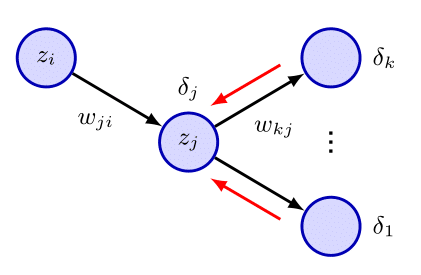
\includegraphics[width=0.7\linewidth]{Plantilla_TFG_latex/imagenes/Mat/Definicion/bp_1.png}
    \caption[Cálculo del error para una unidad oculta ilustando la propagación hacia delante y la propagación hacia atrás del error]{Cálculo del error $\delta_j$ para la unidad oculta $j$ mediante la propagación hacia atrás del error ($\delta$). En la imagen, el nodo $z_j$ representa una neurona en una capa oculta de la red neuronal. Esta neurona recibe una entrada desde otra neurona $z_i$ con un peso sináptico asociado $w_{ji}$ (indicado por la flecha negra). A su vez, la neurona $z_j$ está conectada a varias neuronas $z_k$ en la siguiente capa, con pesos $w_{kj}$. Durante la propagación hacia adelante (flechas negras), la información fluye desde las entradas hacia las salidas de la red. Durante la propagación hacia atrás del error (flechas rojas), los valores de error $\delta_k$ de las neuronas de la capa siguiente se propagan hacia atrás para calcular $\delta_j$, lo que permite ajustar los pesos en función del gradiente del error. Imagen obtenida de \cite{bishop2023learning}.}
    \label{fig:bp_1}
\end{figure}

Con la notación que estamos empleando, cuando $m=1$ el gradiente $\nabla f(x)$ tiene la misma dimensión que $x$. Por tanto es un vector columna mientras que $J_f(x)$ es un vector fila, por lo que técnicamente se tiene que $\nabla f(x)= J_f(x)^T$. Es de vital importancia aclarar esto ya que es el caso en el que nos situamos cuando usamos BP. La dimensión de salida siempre es uno, ya que calculamos la matriz jacobiana de la función de error del modelo con respecto a los pesos, con lo que será un vector gradiente de dimensión igual a la dimensión de los pesos del modelo. La predicción del modelo puede tener dimensión 1 en tareas de regresión, o una dimensión mayor para tareas de clasificación, aunque de manera general no suele ser mayor de 100. La función de error del modelo siempre tendrá como imagen un valor real.


Hemos demostrado que, para el cálculo de una matriz jacobiana, la diferenciación hacia adelante es más eficiente cuando la dimensión de la entrada es menor que la de la salida, mientras que la diferenciación hacia atrás resulta más adecuada cuando la dimensión de la salida es menor que la de la entrada. Dado que en las redes neuronales y los problemas en los que se aplican la dimensión de salida es, por lo general, considerablemente menor que la de entrada, la diferenciación hacia atrás es la opción más eficiente en estos casos.




\subsection{\textit{Backpropagation} en perceptrones multicapa}


En la sección anterior, analizamos un modelo que no tenía parámetros entrenables. Ahora, utilizaremos un modelo que sí los tiene y \textbf{exploraremos cómo calcular el gradiente de la función de coste con respecto a esos parámetros entrenables}. Los parámetros son valores reales y tienen la forma $W= W_1 \times W_2 \times \cdots \times W_k \subset \Omega$, con $W_i \in \mathbb{R}^{n_i \times n_{i+1}}$ donde $n_i$ es el número de neuronas de la $i$-ésima capa. El modelo que tendríamos añadiendo los pesos es $f: \mathbb{R}^n \times \Omega \rightarrow \mathbb{R}^m$, $o=f(x,W)$ con $x \in \mathbb{R}^n$  y $o \in \mathbb{R}^m$. Donde las funciones de cada capa son de la forma $f_i(x_i, W_i)= \sigma_i(W_ix_i)=x_{i+1}$ donde $\sigma_i$ es una función de activación generalmente no lineal. Dependiendo del tipo de problema, la función $f_k$ puede ser distinta: en un problema de regresión usamos la identidad, en clasificación usamos la función \textit{Softmax} que convierte el vector de la predicción del modelo en uno cuyos elementos suman 1 y donde el elemento de la posición $i$-ésima representa la probabilidad de que la entrada pertenezca a la clase $i$.


Ahora vamos a considerar la función de coste del modelo como una capa más de las funciones de las capas ocultas que nos permiten obtener la predicción. Siguiendo con la notación anterior, incluyendo la función de error $\mathcal{L}: \mathbb{R}^n \times \Omega \times \mathbb{R}^m \rightarrow \mathbb{R}$, $E=\mathcal{L}((x,W,y)= C(f(x,W),y)$, con $y \in \mathbb{R}^m$ siendo la etiqueta correcta para la entrada $x$ y $C: \mathbb{R}^m \times \mathbb{R}^m \rightarrow \mathbb{R}$ la función de coste del modelo. Con esto tenemos que $\mathcal{L} = C \circ f$. 

%TODO: revisar porque no he metido los bias a la hora de operar con los pesos del modelo.

\begin{ejemplo}
    Suponemos un MLP con dos capas ocultas, la salida escalar (problema de regresión) y una función de pérdida $C(f(x,W),y)=\frac{1}{2} \| f(x,W) - y\|^2$. Entonces tenemos $\mathcal{L}:\mathbb{R}^n \rightarrow \mathbb{R}$ y cada capa tiene ecuación

    
    
    \begin{gather*}
    f_1(x_1, W_1)=\sigma_1(W_1x_1)=x_2 \\
      f_2(x_2, W_2)=W_2x_2=x_3=f(x,W)=o  \\
      C(f(x,W),y)= \frac{1}{2} \| x_3 - y \|^2 = E
    \end{gather*}

    


\end{ejemplo}

El objetivo será calcular el gradiente del error con respecto a los parámetros $\frac{\partial E}{\partial W}$  para poder utilizarlo el entrenamiento a través del gradiente descendente. Buscamos obtener un vector gradiente de la misma dimensión que $W$, pero el cálculo no es directo, calcularemos progresivamente el gradiente de la función de coste con respecto a los pesos de cada capa, desde la capa final hasta la inicial por lo que buscamos calcular $\frac{\partial E}{\partial W_i}, \forall i=1,\ldots,k$.  Para la última capa $\frac{\partial E}{\partial W_k}$ el cálculo es inmediato, mientras que para el resto podemos usar la regla de la cadena para obtener que 

$$\frac{\partial \mathcal{L}}{\partial W_i}=\frac{\partial \mathcal{L}}{\partial x_k} \frac{\partial x_k}{\partial x_{k-1}} \frac{\partial x_{k-1}}{\partial x_{k-2}} \cdots \frac{\partial x_{i+1}}{\partial W_i}$$

Cada $\frac{\partial \mathcal{L}}{\partial W_i}= \left ( \nabla_{W_i} \mathcal{L}^T \right )$ es un vector gradiente con el mismo número de elementos que $W_i$, es decir, es una submatriz de la matriz jacobiana que contiene los gradientes asociados a los pesos de la capa $W_i$. Estos se calculan propagando hacia atrás la información en el modelo y usando la estrategia de diferenciación hacia atrás a través de PVJ, es decir, el algoritmo de BP que podemos ver en el pseudocódigo del Algoritmo \ref{alg:BPMLPk}. 



\begin{algorithm}
\caption{BP para MLP con k capas}
\label{alg:BPMLPk}
    \begin{algorithmic}
        \State //Propagación hacia delante
        \State $x_1:=x$
        \For{$l \in \left \{1,\ldots,L \right \}$}
            \State $x_{l+1}=f_k(x_l, W_l)$
        \EndFor

        \State //Propagación hacia atrás

        \State $u_{L+1}=1$
        \For{$l \in \left \{L,\ldots,1 \right \}$}
            \State $g_l:= u_{l+1}^T \frac{\partial f_l(x_l, W_l)}{\partial W_l}$
            \State $u_l^T:=u_{l+1}^T\frac{\partial f_l(x_l, W_l)}{\partial x_l}$
        \EndFor
            

        \Return $\left \{  \nabla_{W_l}; l=1,\ldots,L \right \}$
    \end{algorithmic}
\end{algorithm}


Podemos ver una esquematización del proceso en la Figura \ref{fig:bp_2}. Para tener una idea más profunda y completa acerca del algoritmo de BP, vamos a ver cómo calcular el PVJ para las capas más comunes en los modelos, para lo que analizaremos sus matrices jacobianas respecto de la entrada de la capa. 


\begin{figure}
    \centering
    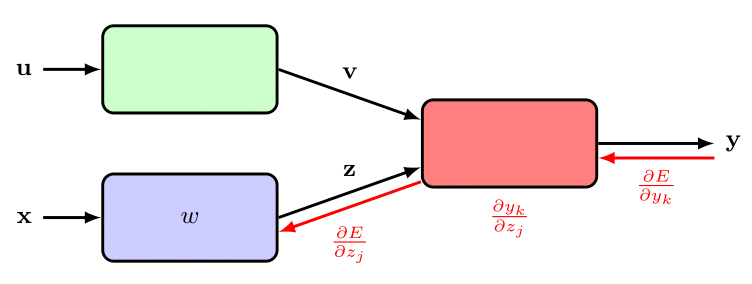
\includegraphics[width=1.0\linewidth]{Plantilla_TFG_latex/imagenes/Mat/Definicion/bp_2.png}
    \caption[Proceso de \textit{backpropagation} en una arquitectura modular de aprendizaje profundo]{Proceso de \textit{backpropagation}, donde una arquitectura modular de aprendizaje profundo en la que la matriz jacobiana se emplea para propagar hacia atrás las señales de error desde las salidas hasta los módulos anteriores en el sistema. En la imagen, las entradas $\mathbf{u}$ y $\mathbf{x}$ se procesan en módulos distintos. El módulo superior recibe $\mathbf{u}$ y produce una salida intermedia $\mathbf{v}$, mientras que el módulo inferior recibe $\mathbf{x}$, con un conjunto de pesos representados por $w$, y genera una salida intermedia $\mathbf{z}$. Ambos valores, $\mathbf{v}$ y $\mathbf{z}$, sirven como entrada para un tercer módulo (en rojo), que produce la salida final $\mathbf{y}$. Durante la propagación hacia atrás del error (indicada por las flechas rojas), la derivada del error con respecto a la salida, $\frac{\partial E}{\partial y_k}$, se propaga hacia atrás a través de la derivada $\frac{\partial y_k}{\partial z_j}$ hasta obtener $\frac{\partial E}{\partial z_j}$. Posteriormente, este error se retropropaga aún más hasta el módulo anterior, permitiendo la actualización de los pesos $w$. Imagen obtenida de \cite{bishop2023learning}.}
    \label{fig:bp_2}
\end{figure}


\subsubsection{Capa no-lineal}



Consideramos primero una capa que aplica una función no lineal, normalmente el caso de las funciones de activación. $z=\sigma(x)$, con $z^{(i)} = \sigma(x^{(i)})$. El elemento en la posición $(i,j)$ del jacobiano es dado por:

$$ \frac{\partial z^{(i)}}{\partial x^{(j)}} =  \left\{\begin{matrix}

\sigma'(x^{(i)}) \quad \textrm{si } i=j  \\
0 \quad \textrm{en otro caso.}
\end{matrix}\right .
$$

Donde $\sigma'(a) = \frac{d\sigma}{da}(a)$. En otras palabras, el jacobiano con respecto de la entrada es 

$$J=\frac{\partial \sigma}{\partial x}= diag(\sigma'(x)).$$

Si tomamos como ejemplo la función \textit{ReLU}, para un vector arbitratio $u$, podemos calcular su PVJ $u^TJ$ a través de la multiplicación  de elementos de la diagonal de $J$ con el vector $u$. 


$$\sigma(a) = ReLU(a)= max(a,0),$$
$$\sigma'(a)=
\left\{\begin{matrix}

0 \quad \textrm{si } a<0  \\
1 \quad \textrm{si } a>0.
\end{matrix}\right.
$$

Como hemos visto en la Sección \ref{sec:subgrad} la función \textit{ReLU} no es diferenciable en el punto 0, pero sí que admite subderivada en todo su dominio, y en el punto $a=0$ es cualquier valor entre $[0,1]$, y usualmente en la práctica se toma el valor 0. Por tanto

$$ReLU'(a)= \left\{\begin{matrix}

0 \quad \textrm{si } a\leq0  \\
1 \quad \textrm{si } a>0 \textrm{.} \\
\end{matrix} \right.$$

$$J=\frac{\partial \sigma}{\partial x}= diag(ReLU'(x)).$$


\subsubsection{Capa de entropía cruzada}

Consideramos ahora la capa cuya función es la función de coste, en concreto con una medición del error usando CE donde tenemos $C$ clases, que toma las predicciones $x$ y las etiquetas $y$ como entrada y devuelve un escalar. Recordamos que en esta capa la matriz jacobiana es un vector fila, identificado con el gradiente, ya que la salida es un escalar.

\begin{align*}
	z&=f(x)=CE(x,y) \\
	&= - \sum_c y_c log(softmax(x)_c) = - \sum_c y_c log(p_c)\\
\end{align*}

donde $p_c=softmax(x)_c= \frac{e^{x_c}}{\sum_{c'=1}^C e^{x_{c'}}}$ son las probabilidades de las clases predichas, e $y$ es la etiqueta correcta con codificación \textit{one-hot encoded vector}, es decir un vector de C elementos que representa la clase real a la que pertenece; si ese elemento pertenece a la clase $k$, todos las posiciones del vector $y$ serán 0 a excepción de la posición $k$, que será 1. El jacobiano con respecto a la entrada es

$$J= \frac{\partial z}{\partial x}= (p-y)^T \in \mathbb{R}^{1\times C}.$$

Vamos a asumir que la clase objetivo es la etiqueta c:

$$z=f(x)=-log(p_c)=-log \left (\frac{e^{x_c}}{\sum_j e^{x_j}} \right ) = log \left ( \sum_j e^{x_j} \right ) - x_c.$$

Entonces

$$\frac{\partial z}{\partial x_i} = \frac{\partial}{\partial x_i} log \sum_j e^{x_j} - \frac{\partial}{\partial x_i}x_c = \frac{e^{x_i}}{\sum_j e^{x_j}} - \frac{\partial}{\partial x_i}x_c = p_i - \mathbb{I}(i=c).$$

\subsubsection{Capa lineal}

Consideramos por último una capa lineal $z=f(x,W)=Wx$, donde $W \in \mathbb{R}^{m \times n}$, con $x \in \mathbb{R}^n$ y $z \in \mathbb{R}^m$ son respectivamente la entrada y la salida de esa capa.

Conviene aclarar, para evitar confusiones, que en la descripción previa hemos considerado las capas ocultas como una combinación de las operaciones lineales que aquí se describen con las funciones de activación, aquí sin embargo las analizamos por separado con el objetivo de una descripción más sencilla y un análisis más individualizado. Esta agrupación es una abstracción y por tanto no varía en cuanto a resultados.


Como $z$ es lineal, el jacobiano de la función de la capa con respecto al vector de entrada de esa capa coincide con su matriz de coeficientes, $\frac{\partial z}{\partial x}=W$

%$$z_i = \sum_{l=1}^n W_{il}x_l.$$

%El elemento que ocupa la posición $(i,j)$ en la matriz jacobiana será 

%$$\frac{\partial z_i}{\partial x_j} = \frac{\partial}{\partial x_j} \sum_{l=1}^n W_{il} x_l = \sum_{l=1}^n W_{il} \frac{\partial}{\partial x_j} x_l = W_{ij}$$

%ya que $\frac{\partial}{\partial x_j} x_l= \mathbb{I} (l=j)$. Por tanto el jacobiano con respecto a la entrada será

%$$J=\frac{\partial z}{\partial x}=W.$$

El PVJ entre $u^T \in \mathbb{R}^{1 \times m}$ y $J \in \mathbb{R}^{m \times n}$ es

$$u^T \frac{\partial z}{\partial x} = u^T W \in \mathbb{R}^{1 \times n}.$$

Ahora consideramos el jacobiano con respecto a la matriz de los pesos, $J=\frac{\partial z}{\partial W}$. Esto se puede representar como una matriz de tamaño $m \times (m \times n)$, que resulta compleja de manejar. Por tanto en lugar de eso veremos de manera individual cómo calcular el gradiente con respecto a un único peso $W_{ij}$. Esto es más sencillo de calcular ya que $\frac{\partial z}{\partial W_{ij}}$ es un vector. Para su cómputo nos fijamos en que 

$$z_l = \sum_{t=1}^n W_{lt}x_t, \qquad \textrm{y}$$

$$\frac{\partial z_l}{\partial W_{ij}} = \sum_{t=1}^n x_t \frac{\partial}{\partial W_{ij}} W_{lt} = \sum_{t=1}^n x_t \mathbb{I}(i=l \textrm{ y } j=t) .$$

Por tanto

$$\frac{\partial z}{\partial W_{ij}} = \left ( 0, \ldots, 0, x_j,  0, \ldots, 0 \right )^T$$

Donde el elemento no nulo ocupa la posición $i$-ésima. El PVJ entre $u^T \in \mathbb{R}^{1 \times m}$ y $\frac{\partial z}{\partial W} \in \mathbb{R}^{m \times ( m \times n)}$ se puede representar como una matriz de tamaño $1 \times (m \times n)$. Vemos que 

$$u^T \frac{\partial z}{\partial W_{ij}}= \sum_{l=1}^m u_l \frac{\partial z_l}{\partial W_{ij}} = u_i x_j.$$

Con lo cual

$$ u^T \frac{\partial z}{\partial W}  = ux^T \in \mathbb{R}^{m \times n}.$$



\subsubsection{Grafos computacionales}

Los MLP son un tipo de Redes Neuronales Profundas donde cada capa se conecta directamente con la siguiente formando una estructura de cadena. Sin embargo,\textbf{ las Redes Neuronales Profundas más recientes combinan componentes diferenciables de forma mucho más compleja, creando un grafo computacional de forma similar a como en la programación se combinan funciones simples para hacer otras más complejas}. La restricción es que el grafo resultante debe de ser un grafo acíclico dirigido, donde cada nodo es una función subdiferenciable. Un grafo acíclico dirigido es un tipo de grafo donde cada arista que une dos nodos tiene un sentido específico desde un nodo al otro (dirigido) y en el que no se forman ciclos, es decir, partiendo de un nodo dado no existe una secuencia de aristas dirigidas por la que se pueda volver a él.



Vamos a ver un ejemplo usando la función $f(x_1,x_2)=x_2e^{x_1}\sqrt{x_1+x_2e^{x_1}}$, cuyo grafo se puede ver representado en la Figura \ref{fig:def.grafo}.


\begin{figure}
    \centering
    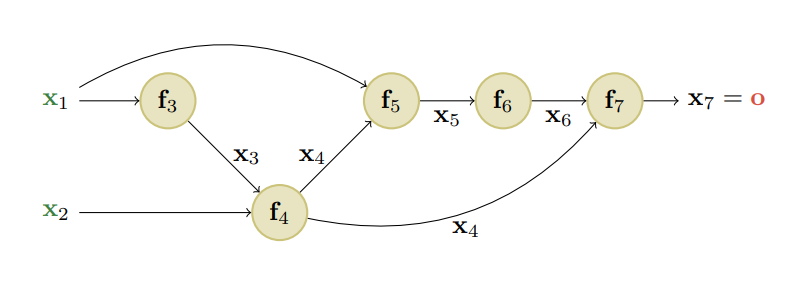
\includegraphics[width=1.0\linewidth]{Plantilla_TFG_latex/imagenes/Mat/Definicion/graf.png}
    \caption[Representación de una red computacional como un grafo dirigido acíclico para diferenciación automática y \textit{backpropagation}]{Representación de una red computacional como un grafo dirigido acíclico para diferenciación automática y BP. La figura muestra un grafo dirigido acíclico donde los nodos representan operaciones matemáticas $f_i$  y las aristas indican el flujo de información entre variables intermedias $x_i$. Las entradas $x_1$ y $x_2$ alimentan las funciones $f_3$ y $f_4$, generando las variables $x_3$ y $x_4$, que a su vez son utilizadas en pasos posteriores. El proceso continúa hasta obtener la salida final $x_7$. Esta estructura permite calcular eficientemente derivadas mediante diferenciación automática en modo de diferenciación hacia atrás, utilizada en el algoritmo de BP para optimizar redes neuronales profundas. Imagen obtenida de \cite{pml1Book}.}
    \label{fig:def.grafo}
\end{figure}


Las funciones intermedias que vemos en el grafo son:

\begin{align*}
x_3= &f_3(x_1)=e^{x_1} \\
x_4 = &f_4(x_2,x_3)=x_2x_3 \\
x_5=&f_5(x_1,x_4)=x_1 + x_4 \\
x_6=&f_6(x_5) = \sqrt{x_5} \\
x_7=&f_7(x_4,x_6)=x_4x_6 .
\end{align*}

Ahora no tenemos una estructura de cadena y en algunos casos necesitaremos sumar los gradientes a través de diferentes caminos, como es el caso del nodo $x_4$ que influye en $x_5$ y $x_7$. Para asegurar un funcionamiento correcto basta con nombrar los nodos en orden topológico (los padres antes que los hijos) y luego hacer la computación en orden topológico inverso. En general usamos

$$ \frac{\partial o }{ \partial x_j } = \sum_{k \in Hijos(j)} \frac{\partial o}{ \partial x_k} \frac{\partial x_k}{\partial x_j}.$$

En nuestro ejemplo para el nodo $x_4$:

$$   \frac{\partial o }{ \partial x_4 }  =  \frac{\partial o}{ \partial x_5} \frac{\partial x_5}{\partial x_4} +\frac{\partial o}{ \partial x_7} \frac{\partial x_7}{\partial x_4} .$$


En la práctica el grafo computacional se puede calcular previamente, usando una librería que nos permita definir un grafo estático. Alternativamente podemos calcular el grafo en tiempo real, siguiendo la ejecución de la función en un elemento de entrada. Esta segunda opción hace más fácil trabajar con grafos dinámicos cuya forma puede cambiar dependiendo de los valores calculados por la función. Por ejemplo, Tensorflow 1 usaba los grafos estáticos mientras que su versión más reciente TensorFlow 2 y PyTorch usan los grafos en tiempo real. 




\subsection{Problemas con el cálculo del gradiente}

\subsubsection{Desvanecimiento y explosión del gradiente}\label{sec:desvyexpl}


Siguiendo el hilo de la Sección \ref{sec:convergencia}, vamos a ver dos problemas que surgen a la hora de entrenar modelos usando gradiente descendente y que pueden impedir la convergencia, pero con la diferencia de que estas limitaciones en la convergencia están ligadas únicamente al algoritmo de BP, es decir, a cómo se calcula el gradiente y no a cómo se usa en la búsqueda de soluciones.

Cuando entrenamos modelos muy profundos (con muchas capas ocultas), los gradientes tienen tendencia bien a volverse muy pequeños (desvanecimiento del gradiente) o bien a volverse muy grandes (explosión del gradiente) ya que la señal de error es pasada a través de una serie de capas que o lo amplifican o lo mitigan. Esto provoca que o bien se deje de actualizar el peso del cual se desvanece su gradiente o que el gradiente diverja en el otro caso \cite{VanishExplode}. Para ver el problema con detalle, consideramos el gradiente de la función de pérdida con respecto a un nodo en la capa $l$:

$$\frac{\partial \mathcal{L}}{\partial z_l} = \frac{\partial \mathcal{L}}{\partial z_{l+1}} \frac{\partial z_{l+1}}{\partial z_l} = g_{l+1} J_l$$

donde $J_l = \frac{\partial z_{l+1}}{\partial z_l}$ es la matriz jacobiana, y $g_{l+1} = \frac{\partial \mathcal{L}}{\partial z_{l+1}}$ es el gradiente de la siguiente capa. Si $J_l$ es constante entre capas, es claro que la contribución del gradiente de la capa final $g_L$ a la capa $l$ será $ g_L J^{L-l}$. Entonces el comportamiento del sistema dependerá de los valores propios de $J$. %TODO: Referencia o explicacion??

$J$ es una matriz de valores reales pero generalmente no es simétrica, por lo que sus autovalores y autovectores pueden ser complejos, representando un comportamiento oscilatorio. Sea $\lambda$ el radio espectral de $J$, que es el máximo del valor absoluto de sus autovalores. \textbf{Si es mayor que 1, el gradiente puede explotar; y si es menor que 1 su gradiente se puede desvanecer. }

El problema de la explosión del gradiente se puede resolver de manera rápida y cómoda a través de acotar el gradiente con su magnitud y una constante $c \in \mathbb{R}^+$ en caso de que se vuelva muy grande

$$g' = min(1, \frac{c}{\|g\|}g)$$

De esta manera la norma de $g'$ nunca puede ser mayor que $c$, pero el vector apunta siempre en la misma dirección que el gradiente.

También existen otras soluciones que además son aplicables al problema del desvanecimiento de gradiente, que no se soluciona de manera tan sencilla:

\begin{itemize}
    \item Adaptar las funciones de activación para prevenir que el gradiente se vuelva muy grande o muy pequeño.

    \item Modificar la arquitectura del modelo para estandarizar las funciones de activación en cada capa, para que la distribución de las activaciones sobre el conjunto de datos permanezca constante durante el entrenamiento.

    \item Elegir cuidadosamente los valores iniciales de los pesos del modelo.
   
\end{itemize}

En la siguiente sección veremos detenidamente el último punto, ya que es la práctica más estandarizada. Existen además familias concretas de modelo que mitigan específicamente estos efectos con su arquitectura como son las ResNets, de las cuales hablaremos en la parte Informática de la memoria.


\subsubsection{Inicialización de los pesos}\label{sec:inipesos}

\textbf{Cómo inicializamos los pesos es una decisión importante a la hora de determinar cómo converge (y si lo hace) un modelo}. La convergencia o no, su velocidad y la solución a la que se converge en el entrenamiento de un modelo mediante el algoritmo de gradiente descendente es muy sensible al punto inicial desde el que comenzamos la búsqueda de una solución. Hay que remarcar que esto sucede cuando la función de error no es convexa, pero como es el caso mayoritario, lo asumimos de manera general.  

Basándonos en \cite{stabilityProblem2}, donde se observa que inicializar parámetros de una distribución normal con varianza fija puede resultar en el problema de la explosión de gradiente, vamos a ver por qué ocurre esto y, a través de añadir restricciones para evitarlo vamos a llegar a las heurísticas de inicialización de pesos más comunes.

Consideramos el pase hacia delante en una neurona lineal sin capa de activación dada por $o_i = \sum_{j=1}^{n_{in}} w_{ij}x_j$ . Suponemos $w_{ij} \sim \mathcal{N}(0, \sigma^2)$, con $\mathbb{E}[x_j]=0$ y $\mathbb{V}[x_j]=\gamma^2$, donde asumimos $x_j$ independiente de $w_{ij}$, y $n_{in}$ es el número de conexiones de entrada que recibe la neurona. La media y la varianza de la salida vienen dadas por

$$\mathbb{E}[o_i]= \sum_{j=1}^{n_{in}} \mathbb{E}[w_{ij} x_j] = \sum_{j=1}^{n_{in}} \mathbb{E}[w_{ij}] \mathbb{E}[x_j]=0$$

$$\mathbb{V}[o_i] = \mathbb{E}[o_i^2] - (\mathbb{E}[o_i])^2 = \sum_{j=1}^{n_{in}} \mathbb{E}[w_{ij}^2x_j^2] - 0 = \sum_{j=1}^{n_{in}} \mathbb{E}[w_{ij}^2] \mathbb{E}[x_j^2] = n_{in} \sigma^2 \gamma^2.$$

Para evitar que la varianza diverja, necesitamos que $n_{in} \sigma^2$ se mantenga constante. Si consideramos el pase hacia atrás y realizamos un razonamiento análogo vemos que la varianza del gradiente puede explotar a menos que $n_{out} \sigma^2$ sea constante, donde $n_{out}$ son las conexiones de salida de la neurona. Para cumplir con esos dos requisitos, imponemos $\frac{1}{2}(n_{in}+n_{out}) \sigma^2 = 1$, o equivalentemente

$$\sigma^2= \frac{2}{n_{in}+n_{out}}.$$

Esta se conoce como inicialización de Xavier o inicialización de Glorot \cite{stabilityProblem2}. Si usamos $\sigma^2= \frac{1}{n_{in}}$ tenemos un caso especial conocida como la inicialización de LeCun, propuesta por Yann LeCun en 1990. Es equivalente a la inicialización de Glorot cuando $n_{in}=n_{out}$. Si usamos $\sigma^2 = \frac{2}{n_{in}}$, tenemos la llamada inicialización de He, propuesta por Kaiming He en \cite{heinic}.


Cabe resaltar que no ha sido necesario usar una distribución Gaussiana. De hecho, las derivaciones de arriba funcionan en términos de la media y la varianza, y no hemos hecho suposiciones sobre si era Gaussiana. 


\textbf{Aunque hemos supuesto que se trataba de una neurona lineal sin función de activación que añada una componente no lineal, se conoce de manera empírica que estas técnicas son extensibles a unidades no lineales}. \textbf{La inicialización que elijamos dependerá mayoritariamente de la función de activación que usemos}. Se conoce que para funciones de activación \textit{ReLU} funciona mejor la inicialización de He, para las funciones \textit{SELU} se recomienda la inicialización de LeCun y para las funciones lineales, logística, tangente hiperbólica y \textit{Softmax} se recomienda el uso de la inicialización de Glorot \cite{pml1Book}.

\newpage

\part{Parte informática: enfoque clásico vs técnicas metaheurísticas}

\vspace{4cm}

\newpage


\input{Plantilla_TFG_latex/Informatica/Introducción}
\section{Experimentación}

Se ha desarrollado una batería de pruebas amplia y diversa que permita una correcta comparación entre el gradiente descendente y las técnicas metaheurísticas atendiendo a los objetivos señalados anteriormente. En la tabla \ref{table:exp} se ofrece un resumen esquemático de las pruebas que se van a realizar. Todas ellas se realizan con los siguientes optimizadores de gradiente descendente: NAG, RMSProp y Adam. Para las metaheurísticas se ha elegido los ya conocidos en la literatura SHADE y SHADE-ILS, y añadiendo una versión híbrida de cada uno con el gradiente descendente. Todas estas elecciones se detallarán a lo largo de esta sección. Para el desarrollo del código se usa el lenguaje Python con las librerías PyTorch y FastAI, entre otras; implementado y ejecutado en Google Colab. El código puede encontrarse en: https://github.com/eedduu/TFG.




\begin{table}[]
\begin{tabular}{|l|cccc|cll|}
\hline
\textbf{Familia} & \multicolumn{4}{c|}{MLP}                                                                                                                               & \multicolumn{3}{c|}{ConvNets}                                         \\ \hline
\textbf{Modelo}  & \multicolumn{4}{c|}{1,2,5 y 11}                                                                                                                        & \multicolumn{3}{c|}{LeNet5, ResNet-15 y ResNet57}                               \\ \hline
\textbf{Datasets}           & \multicolumn{1}{c|}{BHP} & \multicolumn{1}{c|}{BCW} & \multicolumn{2}{c|}{WQ}              & \multicolumn{1}{c|}{MNIST} & \multicolumn{1}{l|}{F-MNIST} & CIFAR10-G \\ \hline
\textbf{Tarea}             & \multicolumn{1}{c|}{R}                        & \multicolumn{1}{c|}{C}            & \multicolumn{1}{c|}{R} & C & \multicolumn{3}{c|}{Clasificación de imágenes}                        \\ \hline
\end{tabular}
\caption{Resumen de la experimentación. BHP: Boston Housing Price, BCW: Breast Cancer Winsconsin, WQ: Wine Quality. R: regresión, C: clasificación. En el caso de MLP, en la fila modelo se indica el número de capas ocultas.}
\label{table:exp}
\end{table}

\subsection{Modelos}

Usaremos dos familias de modelos: MLP y ConvNets. Con los primeros usaremos datasets tabulares para clasificación y regresión, y con los segundos datasets de imágenes para la tarea de clasificación. En la siguiente sección se detallan los datasets con sus características.

La implementación de los MLP se ha realizado a través de la librería FastAI por simplicidad ya que ofrece lo necesario para usarlos directamente. La implementación de las ConvNets se ha realizado desde cero, observando la topología de LeNet5 y las ResNets en sus papers originales, ya que en ellas sí que se han introducido ciertos cambios que se comentan más adelante. Estas modificaciones tienen como objetivo una batería experimental más amplia y acorde a las condiciones que buscamos. Todos los modelos han sido entrenados desde cero.

Para los MLP usaremos 5 modelos, con 1,2,5 y 11 capas ocultas cada uno. El número de neuronas por capa es una potencia de 2 y con estructura piramidal incremental, es decir primero aumentando el número de neuronas por capa y luego disminuyéndolo. Estas son elecciones comunes en la literatura ya que facilitan las operaciones por su estructura (la primera) y el tratamiento de los datos (la segunda). El objetivo es conseguir una variedad experimental que permita medir los efectos de la complejidad del modelo sobre la tarea y el overfitting además de adecuarse a las condiciones del paper de referencia, con modelos desde aproximadamente mil parámetros hasta casi 1.5M como vemos en \ref{tab:MLPmod}, acercándose al modelo más grande presentado en dicho paper. 

\begin{table}[]
\centering
\begin{tabular}{|c|c|c|}
\hline
\textbf{Capas ocultas} & \textbf{Neuronas por capa}                                                                     & \textbf{Parámetros} \\ \hline
1                      & 64                                                                                             & 2238                \\ \hline
2                      & 64, 64                                                                                         & 6462                \\ \hline
5                      & 64, 128, 256, 128, 64                                                                          & 85k                 \\ \hline
11                     & \begin{tabular}[c]{@{}c@{}}32, 64, 128, 256, 512, 1024, \\ 512, 256, 128, 64 y 32\end{tabular} & 1.4M                \\ \hline
\end{tabular}
\caption{Detalles de los modelos MLP}
\label{tab:MLPmod}
\end{table}

Antes de cada capa linal hay una de BatchNorm1D, ya que es la implementación por defecto de FastAI y mejora el rendimiento en el entrenamiento. Los parámetros asociados a este tipo de capa y a los de la capa de salida van incluidos en el cómputo anterior. Se incluye al final del modelo una capa de SoftMax en caso de que la tarea sea clasificación.

Para los modelos basados en convoluciones usamos LeNet5 y dos ResNets, con 15 y 57 capas. El objetivo es de nuevo ofrecer una variedad experimental, con el primer modelo teniendo unos 60k parámetros mientras que el tercero tiene 1.3M, imitando de nuevo las condiciones del paper de referencia. Hay que resaltar que la intención es comparar varios modelos con diferente número de parámetros para ver el efecto sobre éstos, y no hablamos de modelos más o menos potentes, ya que no siempre un incremento en el número de parámetros se traduce en un mejor rendimiento.


LeNet5 es un modelo de sobra conocido presentado por Yann LeCun en \cite{lenet5}, al que sustituimos las funciones de activación por ReLU, ya que en la literatura posterior a la presentación del modelo se han demostrado superiores a las sigmoides y la tangente hiperbólica. También se han sustituido las capas de AveragePool por MaxPool y añadido capas de BatchNorm por los mismos motivos. En la tabla \ref{table:lenet5} se muestra la topología de este modelo, obviando las capas de Flatten y de SoftMax. Tiene un total de 62 mil parámetros.



\begin{table}[]
\centering
\begin{tabular}{|c|c|c|c|}
\hline
\multirow{2}{*}{\textbf{Capa}} & \multirow{2}{*}{\textbf{Dimensión}} & \multirow{2}{*}{\textbf{Kernel}} & \multirow{2}{*}{\textbf{Canales}} \\
                               &                                     &                                  &                                   \\ \hline
Convolución                    & 28x28                               & 5x5                              & 6                                 \\ \hline
BatchNorm2D                    & 28x28                               & -                                & -                                 \\ \hline
ReLU                           & 28x28                               & -                                & -                                 \\ \hline
Max Pool                       & 14x14                               & 2x2, stride 2                    & -                                 \\ \hline
Convolución                    & 10x10                               & 5x5                              & 16                                \\ \hline
BatchNorm2D                    & 10x10                               & -                                & -                                 \\ \hline
ReLU                           & 10x10                               & -                                & -                                 \\ \hline
Max Pooling                    & 5x5                                 & 2x2                              & -                                 \\ \hline
Lineal                         & 120                                 & -                                & -                                 \\ \hline
BatchNorm1D                    & 120                                 & -                                & -                                 \\ \hline
ReLU                           & 120                                 & -                                & -                                 \\ \hline
Lineal                         & 84                                  & -                                & -                                 \\ \hline
BatchNorm1D                    & 84                                  & -                                & -                                 \\ \hline
ReLU                           & 84                                  & -                                & -                                 \\ \hline
Lineal                         & num\_classes                        & -                                & -                                 \\ \hline
\end{tabular}
\caption{Topología de LeNet5 para imágenes 32x32 con un canal de entrada. Las columnas dimensión y canales hacen referencia a la salida de la capa.}
\label{table:lenet5}
\end{table}


Se han diseñado dos modelos de ResNet, uno con 15 capas y otro con 57. A priori puede parecer excesivo 57 capas, pero con la implementación a través de BottleNeckBlocks se aumenta el número de capas considerablemente con un leve incremento del número de parámetros. Sigue además la tendencia en la literatura de aumentar el número de capas antes que el número de filtros. Se han elegido 57 capas con la intención de aproximarse al número de parámetros del modelo más grande del paper de referencia y aprovechar la estructura de esta familia de modelos. Las ResNets se caracterizan por usar bloques convolucionales que agrupan varias capas de convolución donde al final de cada bloque se suma la entrada del mismo, con el objetivo de evitar el problema del desvanecimiento de gradiente (ver sección \ref{sec:desvyexpl}). En un modelo con pocas capas no se aprecia tan bien este efecto. Su topología se detalla en la tabla \ref{table:resnet57}.

El modelo intermedio, Resnet15, sigue la misma estructura que ResNet57 pero usando menos bloques convolucionales. El objetivo es tener un modelo intermedio, con unos 500 mil parámetros y que nos permita comparar con los otros dos, en términos de entrenamiento y de overfitting, algo muy usual en las redes neuronales con gran número de parámetros.  Su topología se detalla en la tabla \ref{table:resnet15}.

Los bloques convolucionales agrupan 3 capas de convolución con sus respectivas capas BatchNorm, y se usan convoluciones 1x1 para hacer cuello de botella, reduciendo así el número de parámetros sin perder expresividad de la red \cite{bottleorig, bottlegoogle}. Se sigue el diseño usual de esta familia de modelos, por ejemplo agrupando más bloques convolucionales en mitad de la red, con una convolución preia a los bloques convolucionales y usando solo una capa lineal. El modelo ResNet57 que se implementa tiene un total de 1.3M de parámetros. 

\begin{table}[]
\begin{tabular}{|c|c|c|c|}
\hline
\multirow{2}{*}{\textbf{Capa}} & \multirow{2}{*}{\textbf{Dimensión}} & \multirow{2}{*}{\textbf{Kernel/Stride}} & \multirow{2}{*}{\textbf{Canales}} \\
                               &                                            &                                         &                                          \\ \hline
Convolución                    & 26x26                                      & 7x7                                     & 64                                       \\ \hline
BatchNorm2d                    & 26x26                                      & -                                       & -                                        \\ \hline
ReLU                           & 26x26                                      & -                                       & -                                        \\ \hline
MaxPool2d                      & 13x13                                      & 2x2, stride 2, padding 1                & -                                        \\ \hline
BottleneckBlock x3             & 13x13                                      & 1x1, 3x3, 1x1                           & 64                                       \\ \hline
BottleneckBlock x4             & 7x7                                        & 1x1, 3x3, 1x1, stride 2                 & 128                                      \\ \hline
BottleneckBlock x4             & 4x4                                        & 1x1, 3x3, 1x1, stride 2                 & 256                                      \\ \hline
BottleneckBlock x3             & 2x2                                        & 1x1, 3x3, 1x1, stride 2                 & 512                                      \\ \hline
AdaptiveAvgPool2d              & 512                                        & -                                       & -                                        \\ \hline
BatchNorm1d                    & 512                                        & -                                       & -                                        \\ \hline
Dropout                        & 512                                        & -                                       & -                                        \\ \hline
Lineal                         & num\_classes                               & -                                       & -                                        \\ \hline
\end{tabular}
\caption{Topología de ResNet57 para imágenes 32x32 con un canal de entrada. Las columnas dimensión y canales hacen referencia a la salida de la capa.}
\label{table:resnet57}
\end{table}


\begin{table}[]
\begin{tabular}{|c|c|c|c|}
\hline
\multirow{2}{*}{\textbf{Capa}} & \multirow{2}{*}{\textbf{Dimensión}} & \multirow{2}{*}{\textbf{Kernel/Stride}} & \multirow{2}{*}{\textbf{Canales}} \\
                               &                                     &                                         &                                   \\ \hline
Convolución                    & 26x26                               & 7x7                                     & 64                                \\ \hline
BatchNorm2d                    & 26x26                               & -                                       & -                                 \\ \hline
ReLU                           & 26x26                               & -                                       & -                                 \\ \hline
MaxPool2d                      & 13x13                               & 2x2, stride 2, padding 1                & -                                 \\ \hline
BottleneckBlock x1             & 13x13                               & 1x1, 3x3, 1x1                           & 64                                \\ \hline
BottleneckBlock x1             & 7x7                                 & 1x1, 3x3, 1x1, stride 2                 & 128                               \\ \hline
BottleneckBlock x1             & 4x4                                 & 1x1, 3x3, 1x1, stride 2                 & 256                               \\ \hline
BottleneckBlock x1             & 2x2                                 & 1x1, 3x3, 1x1, stride 2                 & 512                               \\ \hline
AdaptiveAvgPool2d              & 512                                 & -                                       & -                                 \\ \hline
BatchNorm1d                    & 512                                 & -                                       & -                                 \\ \hline
Dropout                        & 512                                 & -                                       & -                                 \\ \hline
Lineal                         & num\_classes                        & -                                       & -                                 \\ \hline
\end{tabular}
\caption{Topología de ResNet15 para imágenes 32x32 con un canal de entrada. Las columnas dimensión y canales hacen referencia a la salida de la capa.}
\label{table:resnet15}
\end{table}






\subsection{Datasets}

TODO: añadir información sobre los datasets: número de características, target, tamaño, qué contienen, imagenes.

\subsubsection{Tabulares}

BCW y WQ para clasificación, BHP y WQ para regresión. El objetivo es comparar también el rendimiento de las metaheurísticas en estas tareas, ya que la gran mayoría de la literatura sobre MH se realiza con ConvNets y por tanto con tareas de clasificación. BCW y BHP son dos dataset pequeños (alrededor de 500 instancias) y más fáciles que WQ, que tiene una cantidad de unas 6000 instancias. Por ello hay una tarea sencilla y una difícil para regresión y clasificación.

Para estos datasets se ha realizado un preprocesado de los datos básico y con decisiones comunes basadas en la literatura. Se han eliminado las variables que tienen menos de un 5 o 10\% (dependiendo de la cantidad de variables del dataset) de correlación con el target. Con las parejas de variables que tienen más de un 90\% de correlación entre sí se elimina una de las dos. Se han eliminado outliers con el método zscore usando un threshold de 3 y se han normalizado los datos de entrada.

El tamaño del batch se ha elegido mediante pruebas experimentales entre los valores 32, 64 y 128. Se divide el conjunto de datos en entrenamiento-validación-test, con un porcentaje 70-10-20.



\subsubsection{Imágenes}

Para los datasets de imágenes se han elegido tres de los usados en el paper de referencia. Se han elegido MNIST y FMNIST ya que son los más usados para la comparativa en dicho paper, y CIFAR10 ya que a priori es más difícil que los otros, siendo MNIST el más fácil de los tres. Esto proporciona unas pruebas equilibradas, en el mismo marco que el paper y permite una fácil comparación. Al igual que allí, se ha reducido el tamaño de los datasets a 10 mil imágenes para el entrenamiento y 5 mil para el test. Del conjunto de entrenamiento se toma el 30\% para validación.

Se usan las imágenes con una resolución de 32x32 y un solo canal, adaptando las imágenes a estas dimensiones cuando sea necesario. No se usa preprocesamiento de datos ya que se entiende que la propia red a través de las convoluciones los procesa.


\subsection{Otras decisiones}

Para la reproducibilidad de la experimentación, se fija la semilla 42 en todos las librerías necesarias. No se usa cross validation debido a que las técnicas metaheuristicas requieren de mucho más poder de cómputo que el disponible para poder ejecutarlas varias veces en un tiempo razonable.

Se ha usado la inicialización de pesos Glorot  como en el paper a comparar. Para los optimizadores basados en gradiente descendente se han usado los mismos pesos iniciales, mientras que en las técnicas metaheurísticas se ha usado la misma población inicial, para asegurar la igualdad de condiciones en el entrenamiento debido a la gran sensibilidad de éste a los parámetros iniciales. 

Se fija 20 como número de épocas en todos los entrenamientos ya que es suficiente para la convergencia de los métodos de gradiente descendente. Siguiendo el criterio del paper de referencia, en las técnicas metaheurísticas una época es algo distinta, siendo en el paper equivalente a $N_eval * N_epochs * N_capas$. En nuestro caso no se ha usado el factor número de capas por diversas razones: no se realiza entrenamiento individualizado por capas, no se dispone de tanto poder de cómputo, usamos modelos con muchas capas. Aunque usemos menos evaluaciones del conjunto de entrenamiento por época, la comparación sigue en la misma dinámica y las metaheurísticas recibirán mucho más poder de procesamiento que las técnicas clásicas.

Para las tareas de regresión se ha usado el error cuadrático medio como función de coste. Es ampliamente usada en la literatura y aunque es sensible a los outliers, como tenemos preprocesamiento de datos no nos afecta. Se ha usado también la métrica R2 cuadrado para medir la explicación de la varianza con respecto a la media como predicción, para tener un criterio objetivo de comparación ya que en las dos tareas de regresión la escala del objetivo es distinta. Para las tareas de clasificación se ha usado CrossEntropyLoss como función de error y accuracy como métrica, opciones ampliamente usadas en la literatura. En los datasets tabulares se ha usado BalancedAccuracy en lugar de Accuracy, ya que las clases no están balanceadas, y se conoce que en estos casos accuracy no es una métrica representativa, de hecho se hace especial mención a esto en el paper. En los datasets de imágenes las clases están perfectamente balanceadas por lo que se usa accuracy, aunque en este caso su versión balanceada coincidiría con la normal.


\subsection{Optimizadores}

Existen tres familias de optimizadores del gradiente descendente principales: las que usan el momento, las que autoajustan el learning rate y las que combinan estas dos estrategias. Para la experimentación se elige un optmizador de cada familia con la intención de ver si existe alguna diferencia en el entrenamiento del gradiente descendente debido a éstos. El criterio para la elección del optimizador de cada familia ha sido el número de citas en el paper de presentación y su extensión de uso, analizando cómo de frecuente es su uso en la literatura y su implementación por defecto en las principales librerías de aprendizaje automático. Respectivamente se han elegido: NAG, RMSProp y Adam.

Se ha usado la implementación de estos optimizadores de PyTorch, usandose en el entrenamiento a través de la librería FastAI. Se usa en el entrenamiento la política de ciclos de Leslie, que proporciona una velocidad de convergencia mucho mayor variando el learning rate de forma cíclica. Para elegir el valor máximo del learning rate se usa un buscador de learning rate, que aporta unos resultados muy buenos a un coste bajo. Cabe destacar que la importancia del learning rate es sensiblemente menor en los optimizadores de RMSProp y Adam, ya que de manera automática ajustan estos valores a lo largo del entrenamiento. 

Para los hiperparámetros de dichos optimizadores se han usado los valores por defecto de la librería PyTorch. En primer lugar, la intención con la experimentación es establecer una comparativa en igualdad de condiciones sobre el entrenamiento de modelos, y no obtener el máximo rendimiento de cada uno. En segundo lugar estos valores por defecto están basados en los propuestos en los respectivos papers originales y ajustados a través de numerosas pruebas experimentales, de manera que proporcionen los mejores resultados posibles de manera general basandose en la propia implementación de PyTorch. 


\subsection{Metaheurísticas}

Para una correcta comparación con el paper de referencia, que usa el algoritmo SHADE-ILS, se eligen 4 algoritmos metaheurísticos entorno a éste. En primer lugar usamos SHADE-ILS, en su versión completa (entrenando todos los parámetros a la vez). Usamos también el algoritmo de SHADE, sin búsqueda local, para usar un algoritmo puramente metaheurístico que no sea memético. Luego estas dos versiones anteriores las hibridamos con el gradiente descendente, para tener algoritmos meméticos que usen información específica del problema. 

El algoritmo de SHADE se implementa a través de la librería pyade-master (LINK), y se le han realizado modificaciones para mantener los parámetros adaptativos del algoritmo SHADE entre ejecuciones distintas y adaptar las estructuras de datos a las del resto del código. A partir de dicho algoritmo se implementan manualmente el resto. Para el algoritmo SHADE-ILS, que combina dos tipos de búsqueda local en su paper original, con una aplicación general, se ha decidido mantener sólo la búsqueda local a través de L-BFGS, ya que al hacer uso del gradiente se maneja información más específica del problema. Esto se realiza a través de la librería scipy.

Se hibridan SHADE y SHADE-ILS con optimizadores basados en gradiente descendente, aunque SHADE-ILS ya usa información del gradiente en su ejecución a través de L-BFGS pero es un optimizador de segundo orden. Para la hibridación se ejecuta el algoritmo y al final de cada 4 épocas se realiza un entrenamiento de gradiente descendente de una época. Esto se realiza para que el peso del entrenamiento lo siga teniendo en mayor medida la parte metaheurística del algoritmo en lugar de la parte clásica. El optimizador que se usa en este caso es el que mejor resultados diera en el entrenamiento basado en gradiente descendente, eligiendo según el modelo que usemos.  

Se mantiene la misma división de los datos que en el uso de optimizadores. Se ejecutan los algoritmos evaluando el error sobre el conjunto de entrenamiento y guardando en cada epoch el mejor individuo de la población junto a su error en el entrenamiento, para luego evaluarlos sobre el conjunto de validación y observar qué modelo generaliza mejor a priori, igual que hacemos en el entrenamiento de modelos con gradiente descendente. Luego evaluamos el modelo sobre el conjunto de test, calculando las métricas asociadas a cada tarea.

Como en el paper de referencia no aparecen los hiperparámetros asociados a estos algoritmos, se decide usar el mismo criterio que con los optimizadores y usar los hiperparámetros por defecto de la implementación de la librería pyade-master, que además son valores comúnes en la literatura. 












%\part{Parte informática}
%\setcounter{section}{0}
%\vspace{4cm}
%\section{Fundamentos previos}
%\section{Estado del arte}
%\section{Entorno de pruebas}
%PyTorch, fastai, elecciones del entrenamiento, CV, parámetros elegidos en los optimizadores, leslie.

%\paragraph{Elecciones en las pruebas}
%\begin{itemize}

 %   \item NAG, RMSProp y Adam. Uso las 3 estrategias/enfoques distintas en los optimizadores. Uso Nesterov tiene más citaciones su paper. Uso Adam frente a AdamW al tener también más citaciones y ser más comunmente usado. Uso RMSProp frente a AdaGrad ya que generalmente tiene mejor rendimiento (https://arxiv.org/pdf/1609.04747.pdf) (No hay paper para justificar citaciones)

    
  %  \item Entrenamiento con política de leslie. Convergencia más rápida y mayor generalización.

   % \item Grid search para el lr en momentum a partir de los valores devueltos por lr\_find(). En total 4: [lr, lr/10, lr\_steep, lr\_steep/10]. lr\_find() es una buena función para obtener una idea de por donde puede estar el learning rate óptimo. No lo uso en RMSProp ni Adam ya que tienen lr adaptativos y se comenta en papers que no es necesario (https://arxiv.org/pdf/1609.04747.pdf).

    %\item Para el resto de los hiperparámetros seleccionar los valores de los papers originales, en caso de que no haya usar el por defecto de PyTorch. Estos valores para los hiperparámetros se proponen tras muchas pruebas empíricas por lo que suelen ser una buena aproximación en el caso general cuando no se dispone de excesivo tiempo de tunearlos.

    %\item GS para seleccionar batch size, con Valores [64,128,256,512]. 64 es uno de los más usados pero con la política de Leslie mejora la regularización usar batch sizes grandes.

    %\item Para cada ejecución de GS uso 3 epochs. 

    %\item CV 3-fold. Con EarlyStopping de paciencia 3 y delta 0.1 o 0.01. Son valores comunes en la literatura.

    %\item Experimentación modular, orden de realización de experimentos:
     %   \begin{enumerate}
      %      \item LeNet5 con MNIST y CIFAR-10.

       %     \item Algoritmo genético. 

        %    \item ResNet18 con MNIST y CIFAR-10.

         %   \item Algoritmo memético

          %  \item Añadir más datasets

           % \item Probar variaciones en el genético/memético
        %\end{enumerate}
    
%\end{itemize}


%\subsection{Modelos}
%Describir los modelos usados
%\subsection{Datasets}
%Describir los datasets usados
%\section{Análisis de los métodos clásicos}
%Comentar los 3 optimizadores que uso, su base teórica y puntos fuertes y deficiencias de cada estrategia. 

%\paragraph{Momento}

%\paragraph{Learning Rates adaptativos}

%\paragraph{Combinación}

%\subsection{Resultados experimentales}
%Comparación del rendimiento de los 3 en las distintas pruebas. 

%\section{Nuevos enfoques y metaheurísticas}
%Comentar cuándo se empezaron a usar en ML, en qué tareas se les da mejor y en cuales se usan más. Comentar distintos tipos de metaheuristicas, enfocando en algoritmos geneticos que son los más usados y que mejor resultado dan de manera general en problemas de optimización , pero que suelen llevar a un overffiting en entrenamiento. Aun asi se usan para arquitecturas y seleccion de hiperparámetros.

%En principio los algoritmos geneticos sobreentrenan los modelos por tanto no hacer prueba empírica de un genético estándar, sino realizar trabajo teorico de ellos como de otras alternativas basadas en distintas metaheurísticas. Prueba empírica con propuesta. Poner ejemplos concretos de trabajos realizados, resultados, problemas, puntos fuertes y debiles, investigaciones futuras.


%\subsection{Propuesta} 
 %La mayoria de algoritmos geneticos se entrenan con todos los pesos a la vez sin hacer distincion por capas (Lights and Shadows in Evolutionary Deep Learning: Taxonomy, Critical Methodological Analysis, Cases of Study, Learned Lessons, Recommendations and Challenges), en este mismo paper se usa entrenamiento basado en evolutivos pero entrenando primero una capa mientras están las demás fijas. Proponer una variacion de algoritmo genetico con un nivel más de abstracción donde la representacion sea de: individuo=modelo, cromosoma=capa, gen=peso de la capa; aquí la recombinación no sería entre dos genes sino entre dos cromosomas. No he visto representaciones de este tipo en la literatura, aunque debería hacer una búsqueda más exhaustiva para asegurarme. A mi parecer esta representación se parece más al proceso de evolución (una persona tiene varios cromosomas cada uno con sus genes, y cada dos cromosomas del mismo tipo combinan sus genes). Además debido a la estructura de los modelos en FastAI y Pytorch resulta sencillo de operar con ellos de esta manera (a traves de un objeto learner). Usar para la recombinación el operador BLX-$\alpha$. Esto sería equivalente a usar una representación de un vector real pero usando el operador BLX-$\alpha$, en lugar de sobre cada valor independientemente, sobre un conjunto fijado de valores. El seleccionar esos conjuntos como las capas tiene bastante sentido a nivel semántico y mete una abstracción de alto nivel, que podría resultar beneficiosa. Al realizar modificaciones de la capa en su conjunto en lugar de a cada peso, la restricción es mayor y podría servir de regularizacion. Se estarían mejorando filtros en su conjunto en lugar de valores individuales.

%Los demás detalles serán a concretar tras la experimentación, pero en principio selección por torneo es ampliamente usado y no costoso. El número de la población suele situarse en 50, si uso un valor cercano a ese haría un modelo estacionario para ahorrar computación, podría probar con modelo generacional si uso un valor más bajo como 5 o 10. Idea para la mutación: truncamiento de valores float a un número concreto de decimales, simulando la imperfección en la copia genética, sería una mutación general (actúa sobre todo el cromosoma o individuo en lugar de sobre un gen concreto) que se iría acumulando de a poco. Previsiblemente el coste computacional no será todo lo reducido que debiera por el uso del objeto learner en lugar de estructuras de datos de bajo nivel, pero creo que si me pongo a realizar esas cosas de bajo nivel sería demasiado costoso y puede salir mal.


%Proponer otra variación basado en meméticos: cada x generaciones se realiza un entrenamiento de los modelos usando GD. De esta manera se combina la capacidad exploradora (busqueda global) de los genéticos con la capacidad explotadora (busqueda local) del gradiente descendente. 

%\subsection{Resultados experimentales}
%\section{Conclusiones}





%
%\input{capitulos/02_EspecificacionRequisitos}
%
%\input{capitulos/03_Planificacion}
%
%\input{capitulos/04_Analisis}
%
%\input{capitulos/05_Diseno}
%
%\input{capitulos/06_Implementacion}
%
%\input{capitulos/07_Pruebas}
%
%\input{capitulos/08_Conclusiones}
%
%%\chapter{Conclusiones y Trabajos Futuros}
%
%
%%\nocite{*}

\addcontentsline{toc}{section}{Bibliografía}
\newpage
\printbibliography
%\bibliographystyle{miunsrturl}
%
%\appendix
%\input{apendices/manual_usuario/manual_usuario}
%%\input{apendices/paper/paper}
%\input{glosario/entradas_glosario}
% \addcontentsline{toc}{chapter}{Glosario}
% \printglossary
%\chapter*{}
%\thispagestyle{empty}

\end{document}
